\documentclass[]{beamer}
\usepackage{beamerthemesplit}
\usepackage{graphics,epsfig}
\usepackage{pstricks}
\usepackage{graphicx}
\usepackage{amsmath}
\usepackage{amssymb}
\usepackage{hyperref}
\usepackage{subfigure}
\usepackage{multirow}
\usepackage{xspace}
\usepackage{listings}
\usepackage{algorithm}
\usepackage{algorithmicx}
\usepackage{tikz}
\usepackage{algpseudocode}
\usepackage{xcolor}

\mode<presentation>
{ \usetheme{CambridgeUS}
  \setbeamercovered{transparent}
  \setbeamertemplate{items}[circle]
  \setbeamertemplate{theorems}[numbered]
%  \setbeamertemplate{footline}[frame number]
}


\makeatletter
\definecolor{cornblue}{HTML}{6495ED}
\definecolor{navyblue}{HTML}{000080}
\definecolor{midnblue}{HTML}{191970}
\definecolor{lghtblue}{HTML}{B0C4DE}
\setbeamercolor{background}{fg=black, bg=lghtblue}
%\setbeamercolor{palette primary}{fg=white, bg=lghtblue}
\setbeamercolor{palette secondary}{fg=black, bg=cornblue}
\setbeamercolor{palette tertiary}{fg=black, bg=lghtblue}
\setbeamercolor{palette quaternary}{fg=black, bg=lghtblue}
\setbeamercolor{frametitle}{fg=midnblue, bg=white}


\useinnertheme[shadow=true]{rounded}
\useoutertheme{shadow}
\usecolortheme{whale}

\newcommand\blfootnote[1]{
  \begingroup
  \renewcommand\thefootnote{}\footnote{#1}
  \addtocounter{footnote}{-1}
  \endgroup
}



\makeatletter


\mode
<all>

\author[Wan-Lei Zhao]{WanLei Zhao}
\title{Multimedia Technology}

\makeatletter
\DeclareRobustCommand\onedot{\futurelet\@let@token\@onedot}
\def\@onedot{\ifx\@let@token.\else.\null\fi\xspace}
\makeatother

\begin{document}
\begin{frame}
   \begin{center}
    \vspace{24pt}
    \Huge\textbf{Multimedia Technology}\blfootnote{Email: wlzhao@xmu.edu.cn, \textit{copyrights are fully reserved by the author.}}\\
     \Large{\mbox{Lecture 6: Fundamentals about Image Processing}}
    \vspace{36pt}
  \end{center}
  \begin{align*}
   \vspace{18pt}
      \large{\mbox{Lecturer:}~Dr.~\mbox{Wan-Lei~~Zhao}} \\
      \large{Autumn~~Semester~~2022} \\
   \vspace{30pt}
  \end{align*}
\end{frame}



\definecolor{ballblue}{rgb}{0.13, 0.67, 0.8}
\definecolor{cornflowerblue}{rgb}{0.39,0.58,0.93}
\definecolor{babyblueeyes}{rgb}{0.63, 0.79, 0.95}

% preset-listing options
\lstset{
  backgroundcolor=\color{white},   
  basicstyle=\normalsize,    
  language=html,
  breakatwhitespace=false,         
  breaklines=true,                 % sets automatic line breaking
  captionpos=b,                    % sets the caption-position to bottom
  commentstyle=\color{ballblue},    % comment style
  extendedchars=true,              
  frame=single,                    % adds a frame around the code
  keepspaces=true,                 
  keywordstyle=\color{blue},       % keyword style
  numbers=left,                    
  numbersep=5pt,                   
  numberstyle=\tiny\color{blue}, 
  rulecolor=\color{babyblueeyes},
  stepnumber=1,              
  stringstyle=\color{black},     % string literal style
  tabsize=4,                       % sets default tabsize to 4 spaces
  title=\lstname                   
}


\section{Fundamentals about Image}
\begin{frame}<beamer>
    \frametitle{Outline}
    \tableofcontents[currentsection]
\end{frame}

\begin{frame}
 \frametitle{Opening Discussion (1)}
 \begin{itemize}
 	\item {From now on, we are going to explore a new field}
 	\item {Image and Videos}
 	\item {It is another dimension of Multimedia}
 	\item {In our daily life, around \textbf{80\%} information comes from vision}
 	\item {With the proliferation of digital devices, millions of images/videos are generated each day}
 \end{itemize}
 \begin{figure}
 \begin{center}
	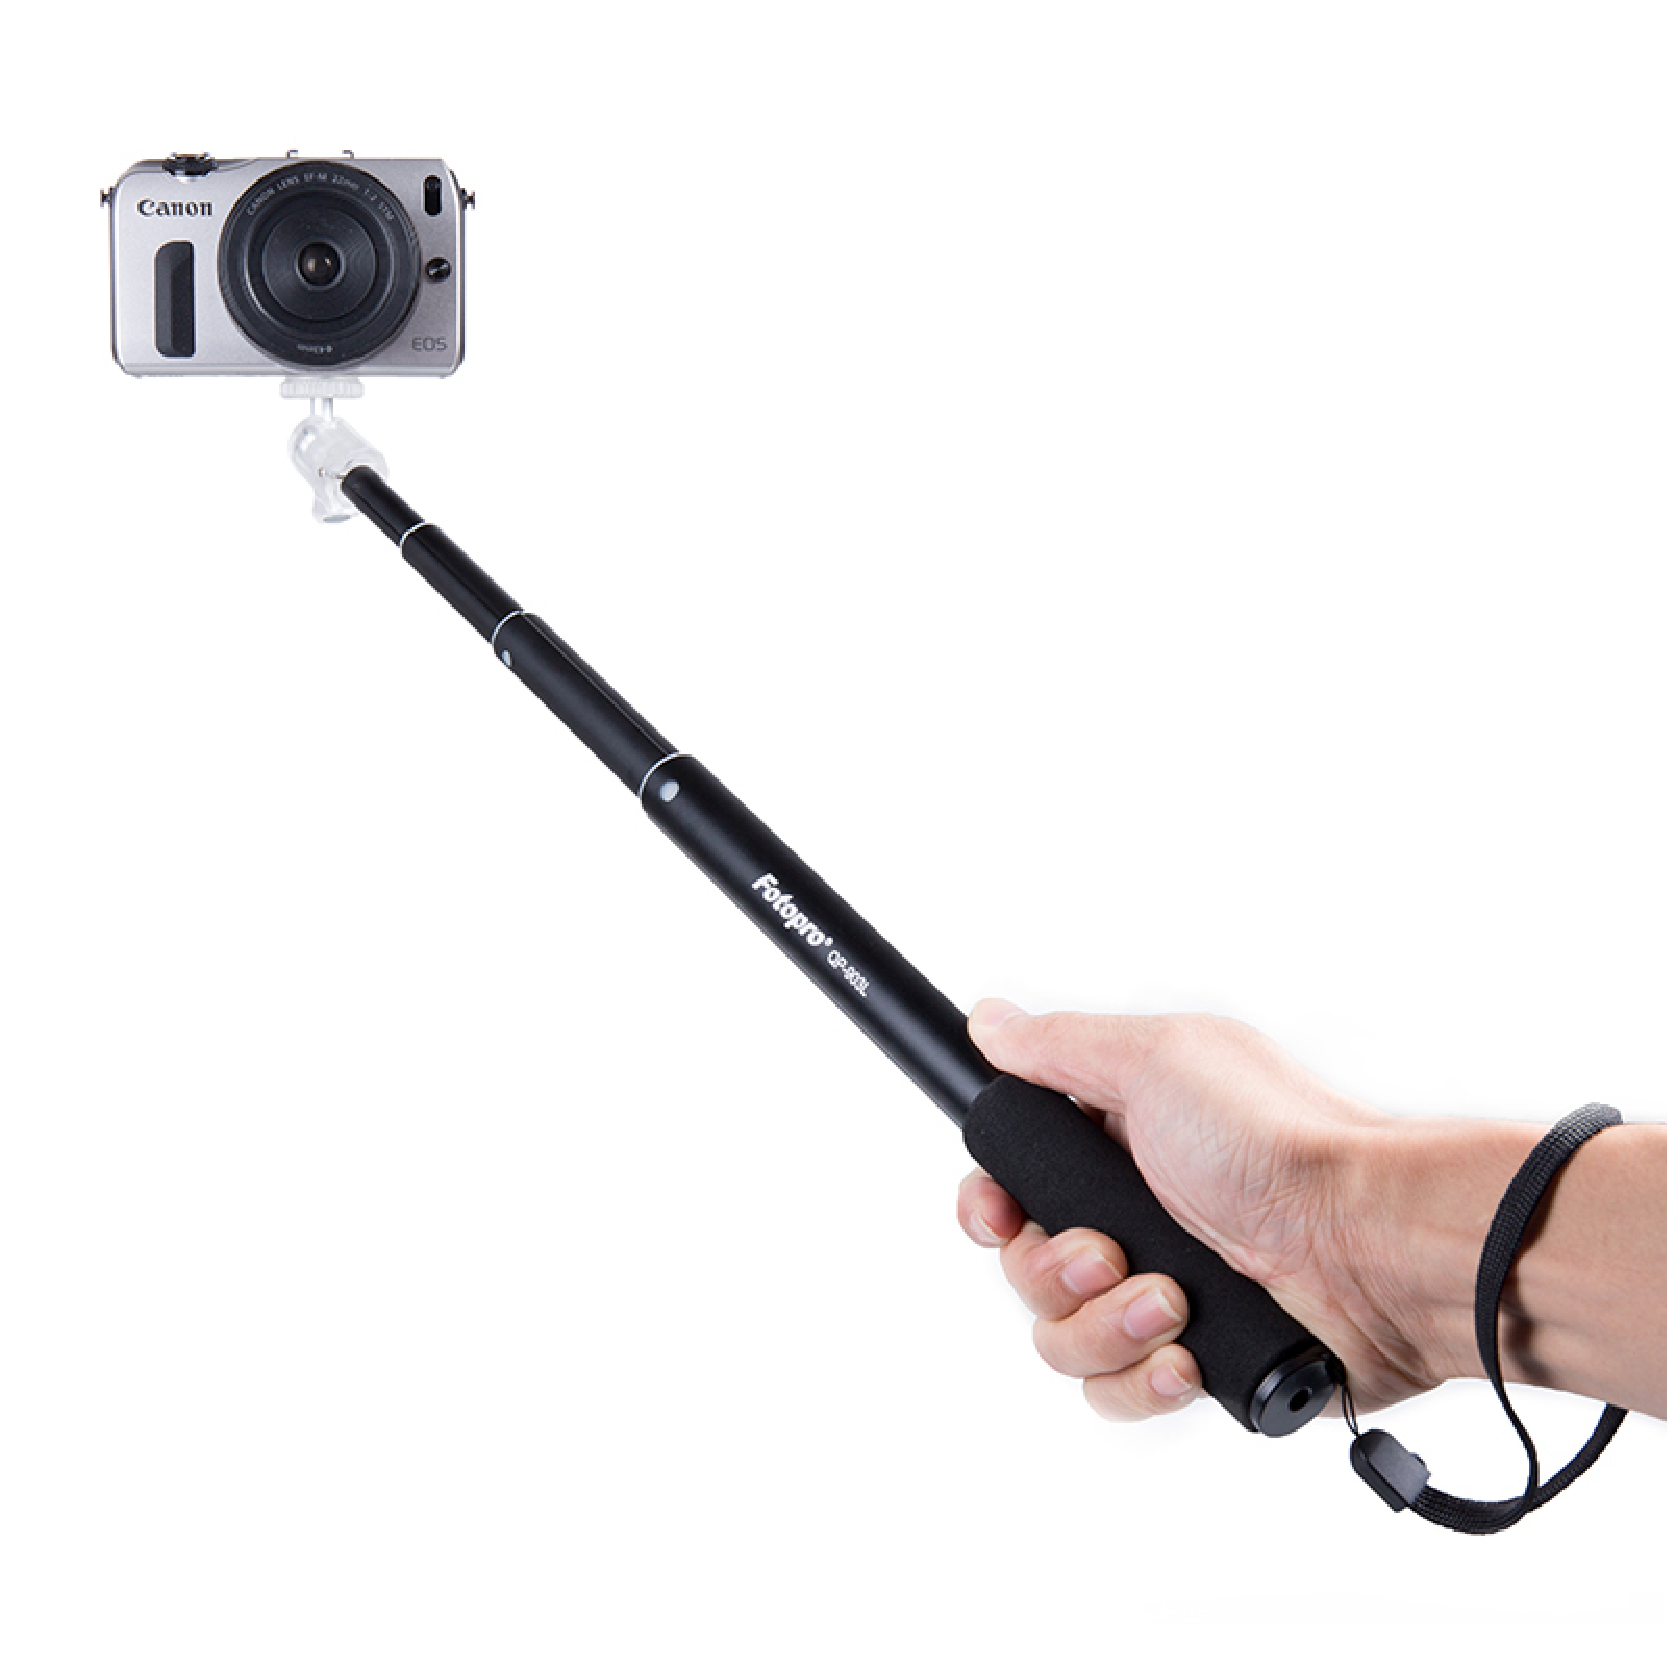
\includegraphics[width=0.350\linewidth]{./figs/support.pdf}
 \end{center}
 \end{figure}
\end{frame}
 
\begin{frame}
 \frametitle{Opening Discussion (2)}
\begin{itemize}
 	\item {It was \textcolor{red}{guessed} that vision caused \textbf{Cambrian Explosion} which took place in 542 million years ago}
 	\item {Vision drove all creatures to evolve faster to survive}
 	\item {With vision, they could search for food easier than before}
 \end{itemize} 
 \begin{figure}
\begin{center}
	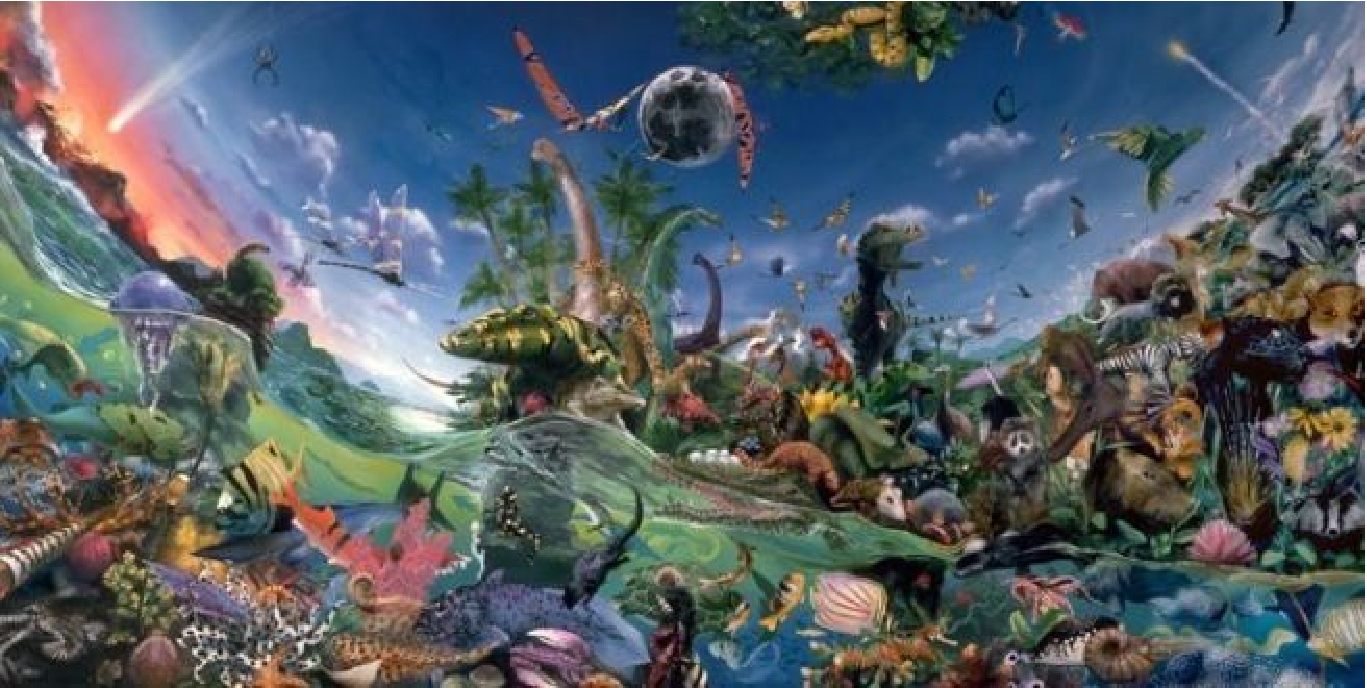
\includegraphics[width=0.80\linewidth]{./figs/cambrian.pdf}
\end{center}
\end{figure}

\end{frame}

\begin{frame}
 \frametitle{Brief history about Digital Image (1)}
 \begin{itemize}
 	\item {It was a long dream that one day we could keep what we see in somewhere besides our brain}
 \end{itemize}
 \begin{figure}
\begin{center}
	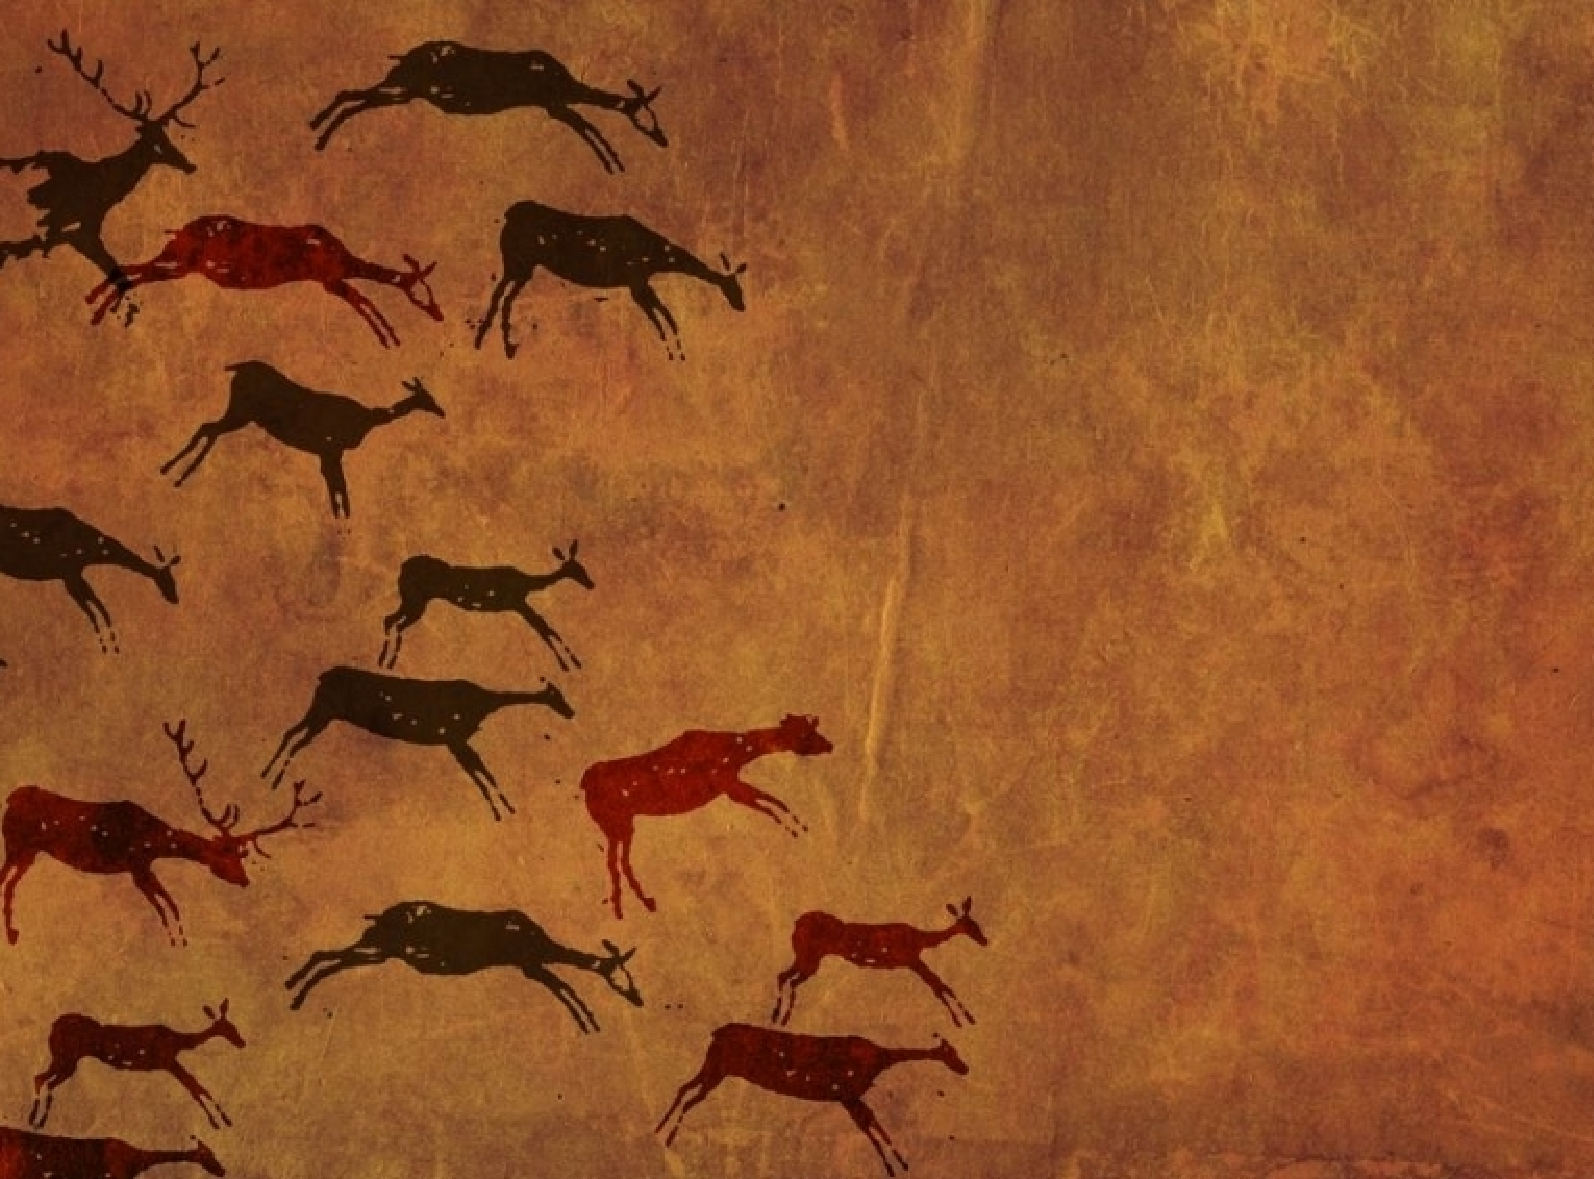
\includegraphics[width=0.6\linewidth]{./figs/neanderthal_paint.pdf}
\end{center}
\caption{Painting by Neanderthal who lived in Europe around 40,000 years ago.}
\end{figure}
\end{frame}

\begin{frame}
 \frametitle{Brief history about Digital Image (2)}
 \vspace{-0.1in}
 \begin{figure}
\begin{center}
	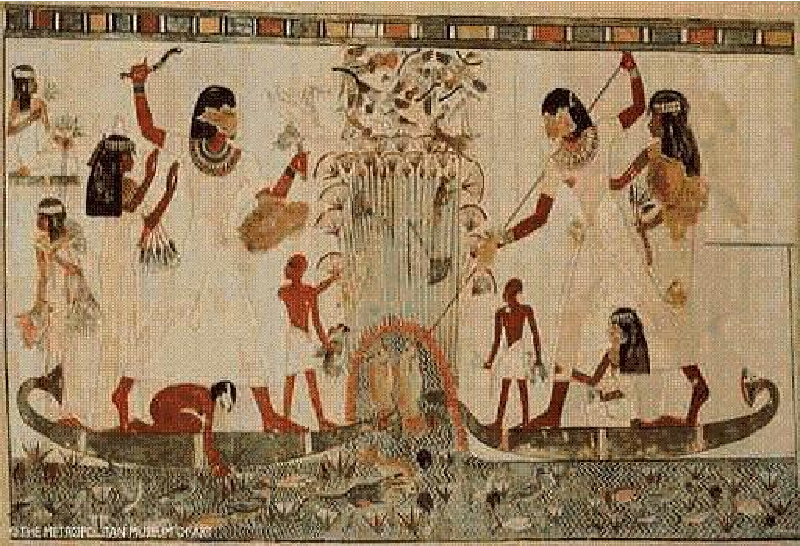
\includegraphics[width=0.66\linewidth]{./figs/egypt_paint.pdf}
\end{center}
\caption{Painting by ancient Egyptian who lived in 5,000 years ago.}
\end{figure}
 \begin{itemize}
 	\item {Notice that in these two periods, people could only try to draw what they saw}
 \end{itemize}
\end{frame}

\begin{frame}
 \frametitle{Brief history about Digital Image (3)}
 \begin{figure}
\begin{center}
	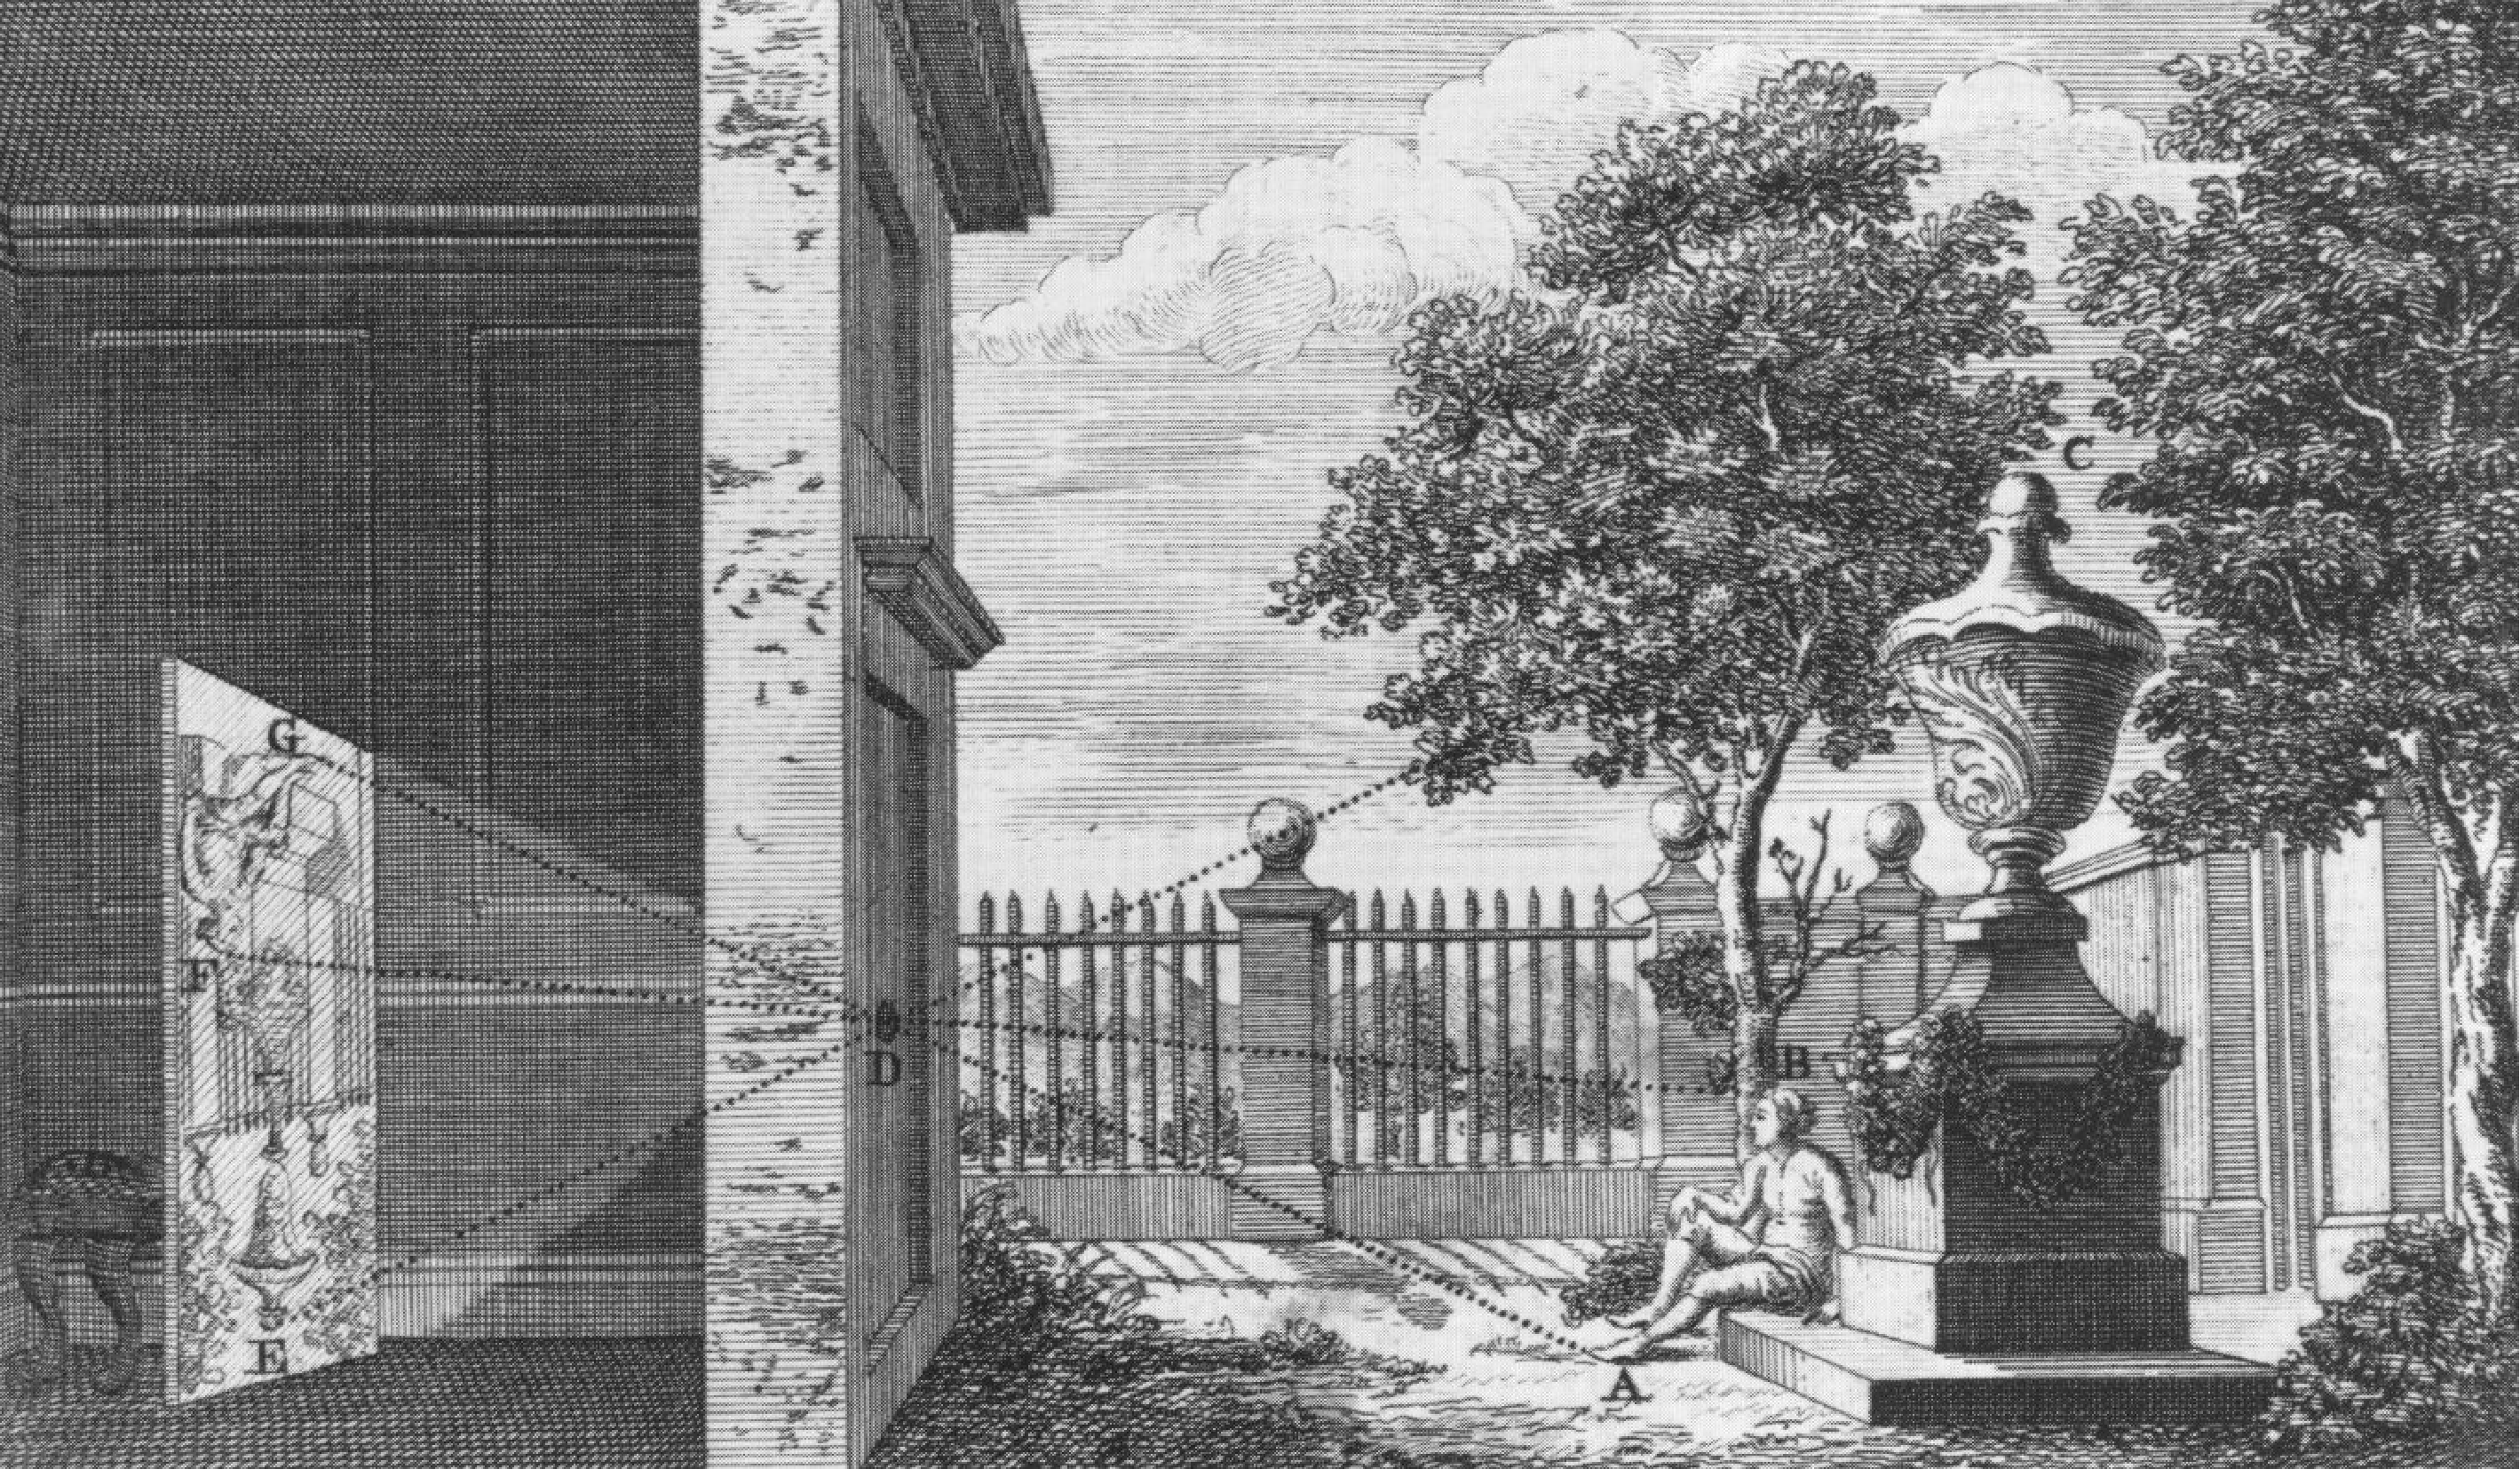
\includegraphics[width=0.66\linewidth]{./figs/camera_obscura.pdf}
\end{center}
\caption{The known first camera by Aristotle.}
\end{figure}
 \begin{itemize}
 	\item {Why it works?}
 	\item {How the size of aperture impacts the projected image}
 	\item {How to keep this capture is still a big problem}
 \end{itemize}
\end{frame}

\begin{frame}
 \frametitle{Brief history about Digital Image (4)}
\vspace{-0.1in}
\begin{figure}
\begin{center}
	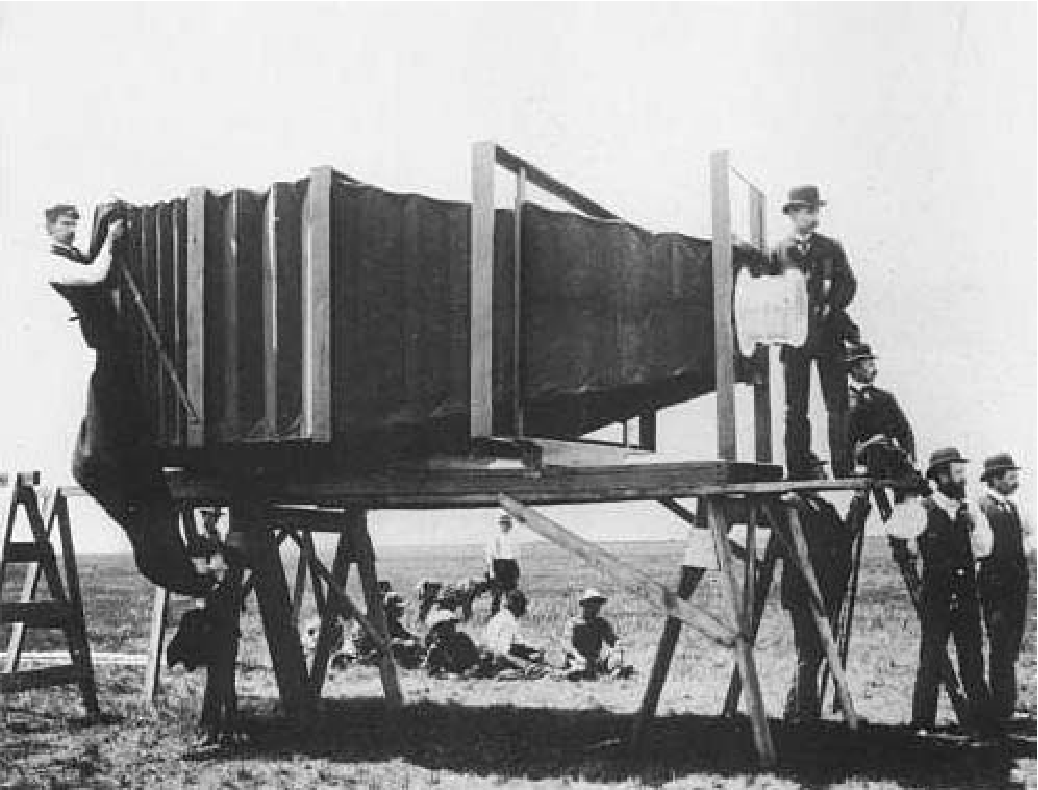
\includegraphics[width=0.53\linewidth]{./figs/biggest_camera.pdf}
\end{center}
\caption{In 1900 the Chicago \& Alton Railroad Train co. , commissioned Lawrence with the manufacture of the largest camera ever made and the largest photo ever shot in order to promote a new train.}
\end{figure}
\vspace{-0.1in}
\begin{itemize}
	\item {Around 30 years before that event, film was invented}
	\item {However, it requires long time of exposure}
\end{itemize}
\end{frame}

\begin{frame}
 \frametitle{Basic knowledge about camera}
  \vspace{-0.1in}
\begin{figure}
\begin{center}
	{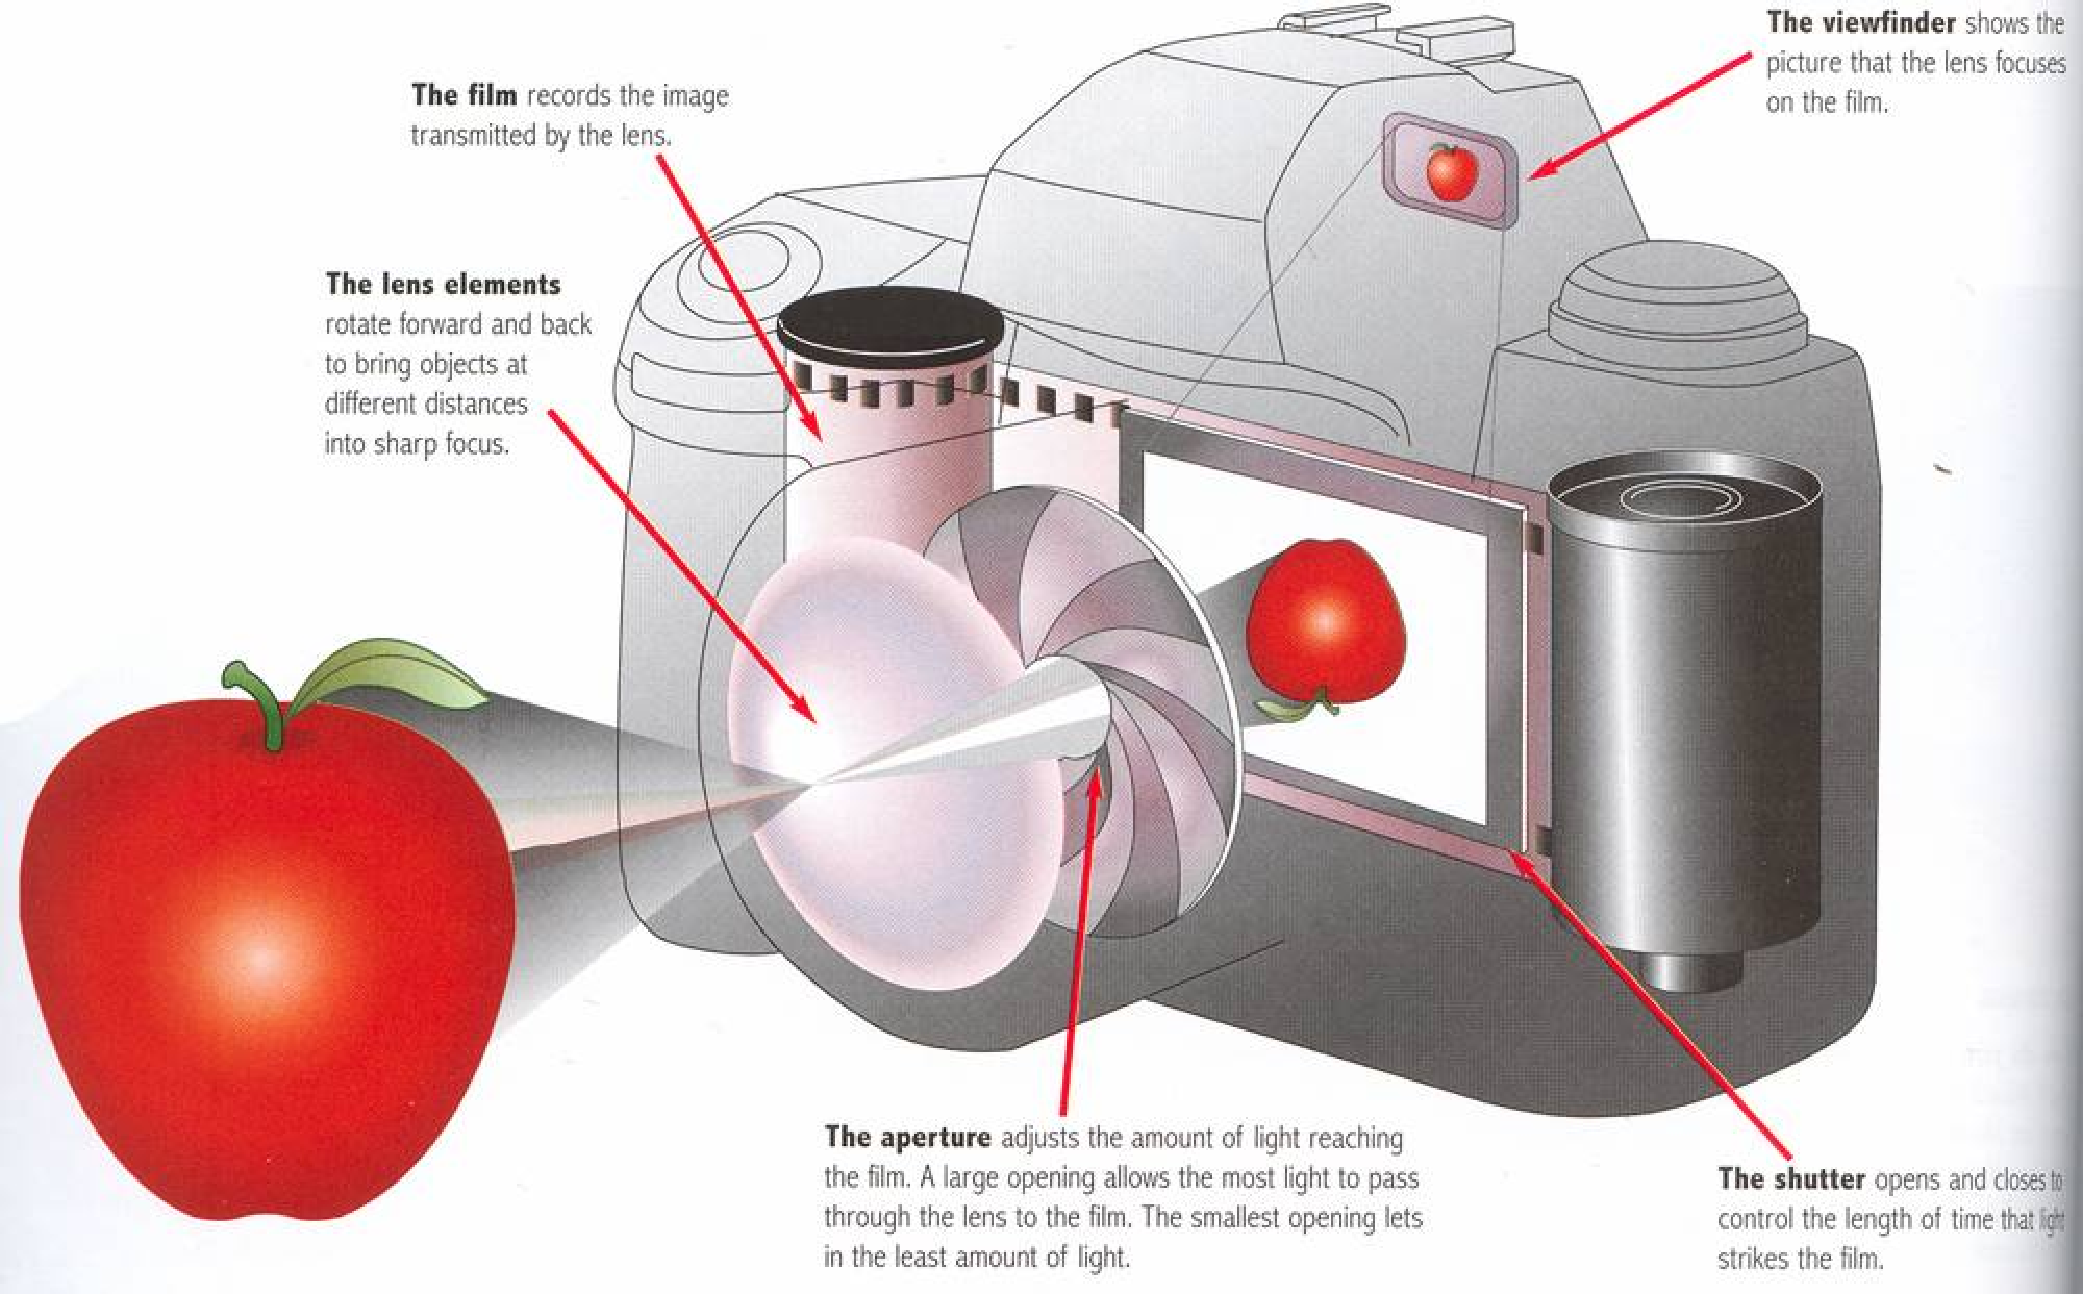
\includegraphics[width=0.55\linewidth]{./figs/camera.pdf}}
\end{center}
\caption{Structure of a modern camera}
\end{figure}

\begin{itemize}
	\item {Major components}
	\begin{enumerate}
		\item {Lens}
		\item {Aperture}
		\item {Film/Sensor field}
	\end{enumerate}
\end{itemize}

\end{frame}


\begin{frame}
 \frametitle{Basic knowledge about camera: the lens (1)}
  \vspace{0.2in}
\begin{figure}
\begin{center}
	{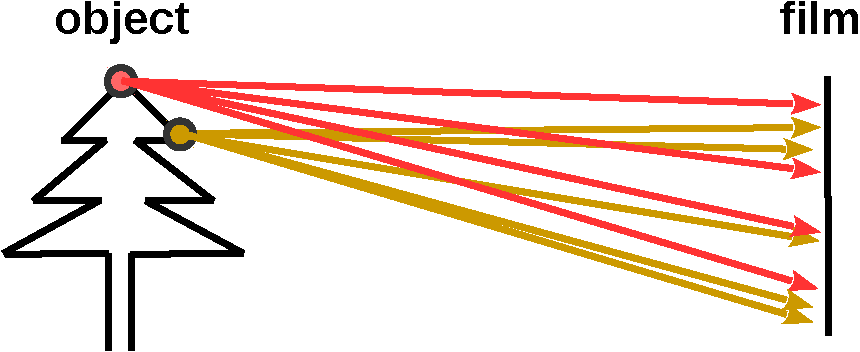
\includegraphics[width=0.5\linewidth]{./figs/holeno.pdf}}
\end{center}
\caption{Try to put film in front of an object, see what you can get}
\end{figure}
\begin{itemize}
	\item {You get nothing but gray because ambient lights come from all directions}
\end{itemize}
\end{frame}


\begin{frame}
 \frametitle{Basic knowledge about camera: the lens (2)}
  \vspace{-0.1in}
\begin{columns}
\begin{column}{0.35\linewidth}
\begin{figure}
\begin{center}
	{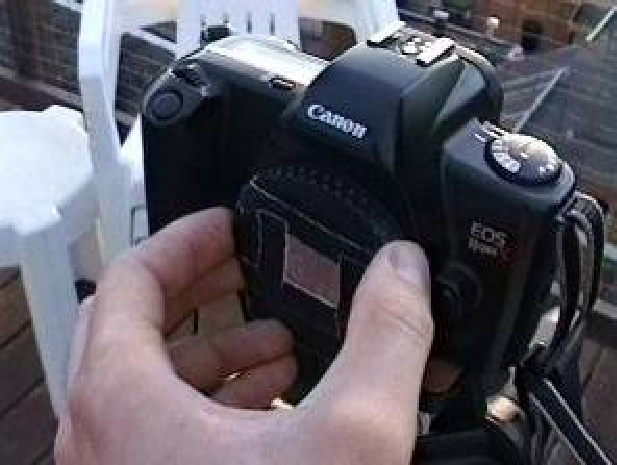
\includegraphics[width=0.75\linewidth]{./figs/removelens.pdf}}
\end{center}
\caption{Remove camera lens}
\end{figure}
\begin{itemize}
	\item {Why blurry??}
\end{itemize}
\end{column}
\begin{column}{0.65\linewidth}
\begin{figure}
\begin{center}
	{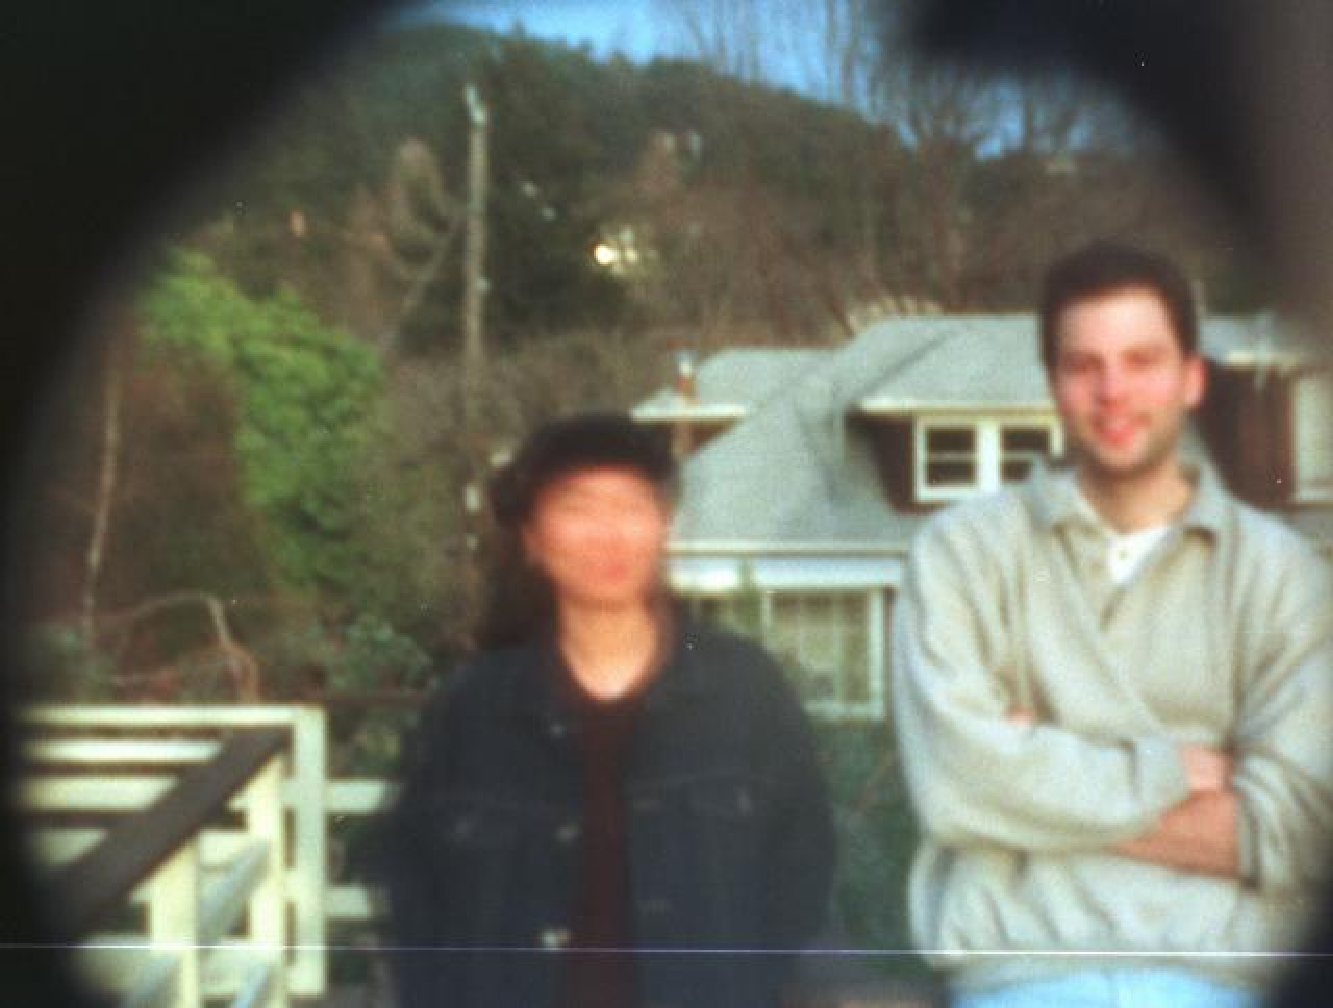
\includegraphics[width=0.95\linewidth]{./figs/photonolens.pdf}}
\end{center}
\caption{Camera imaging without lens.}
\end{figure}
\end{column}
\end{columns}
\end{frame}


\begin{frame}
 \frametitle{Basic knowledge about camera: the lens (3)}
  \vspace{-0.1in}
\begin{figure}
\begin{center}
	\subfigure[2mm]
	{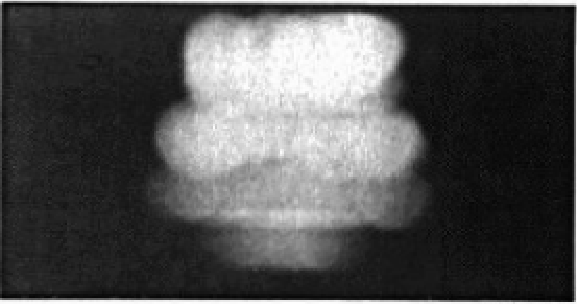
\includegraphics[width=0.25\linewidth]{./figs/hole2mm.pdf}} \hspace{0.08in}
	\subfigure[1mm]
	{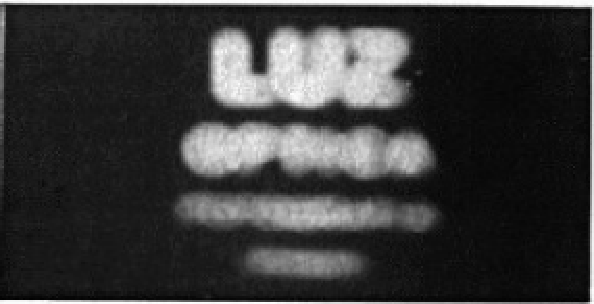
\includegraphics[width=0.25\linewidth]{./figs/hole1mm.pdf}} \\
	\subfigure[0.6mm]
	{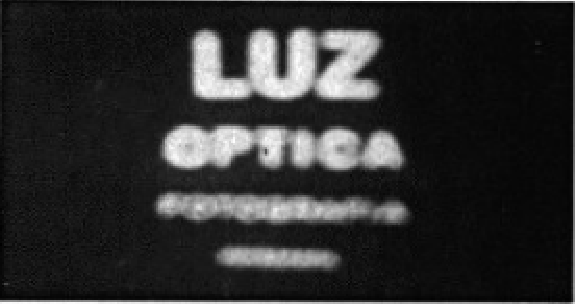
\includegraphics[width=0.25\linewidth]{./figs/hole06mm.pdf}} \hspace{0.08in}
	\subfigure[0.35mm]
	{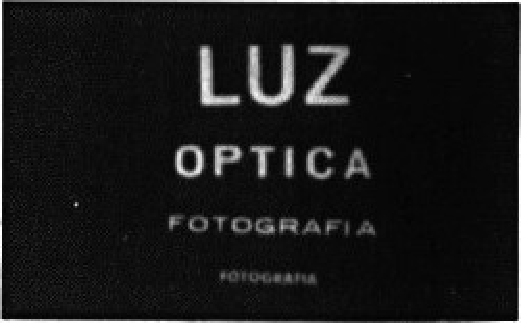
\includegraphics[width=0.25\linewidth]{./figs/hole035mm.pdf}}\\ 
\end{center}
\caption{Imaging with different sizes of hole.}
\end{figure}
\begin{itemize}
	\item {Is it the smaller the better?}
\end{itemize}
\end{frame}

\begin{frame}
 \frametitle{Basic knowledge about camera: the lens (4)}
 \vspace{-0.1in}
\begin{figure}
\begin{center}
	\subfigure[2mm]
	{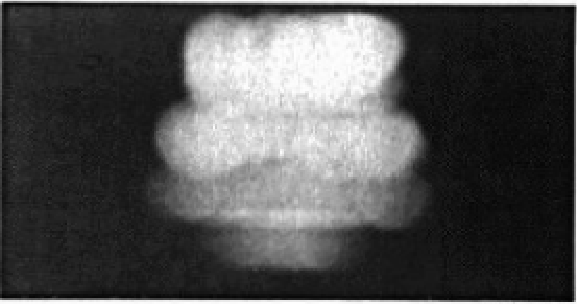
\includegraphics[width=0.25\linewidth]{./figs/hole2mm.pdf}} \hspace{0.08in}
	\subfigure[1mm]
	{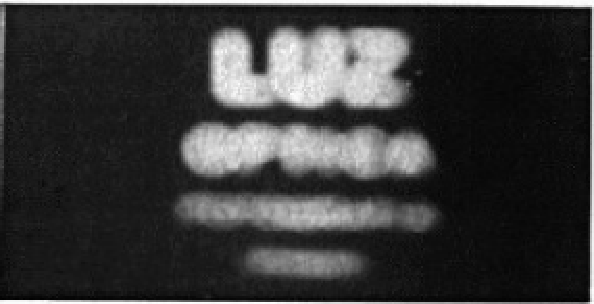
\includegraphics[width=0.25\linewidth]{./figs/hole1mm.pdf}} \\
	\subfigure[0.6mm]
	{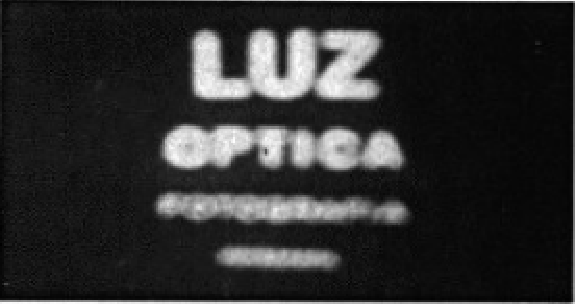
\includegraphics[width=0.25\linewidth]{./figs/hole06mm.pdf}} \hspace{0.08in} 
	\subfigure[0.35mm]
	{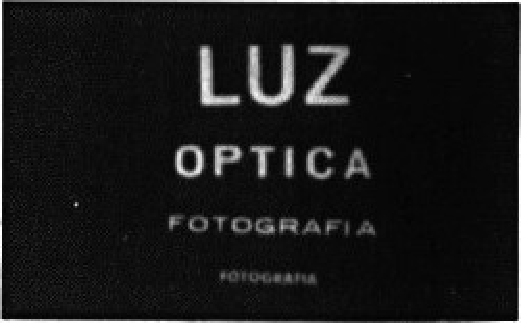
\includegraphics[width=0.25\linewidth]{./figs/hole035mm.pdf}}\\ 
	\subfigure[0.17mm]
	{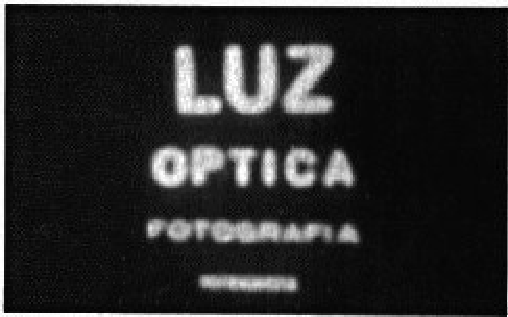
\includegraphics[width=0.25\linewidth]{./figs/hole015mm.pdf}} \hspace{0.08in}
	\subfigure[0.07mm]
	{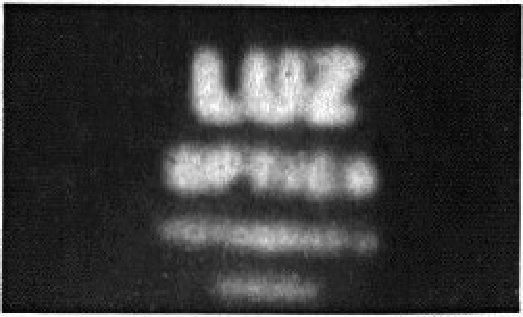
\includegraphics[width=0.25\linewidth]{./figs/hole007mm.pdf}}
\end{center}
\caption{Imaging with different sizes of hole.}
\end{figure}
\end{frame}

%\begin{frame}
% \frametitle{Basic knowledge about camera: the lens (5)}
% \begin{columns}
% \begin{column}{0.6\linewidth}
% \vspace{-0.20in}
%\begin{figure}
%\begin{center}
%	{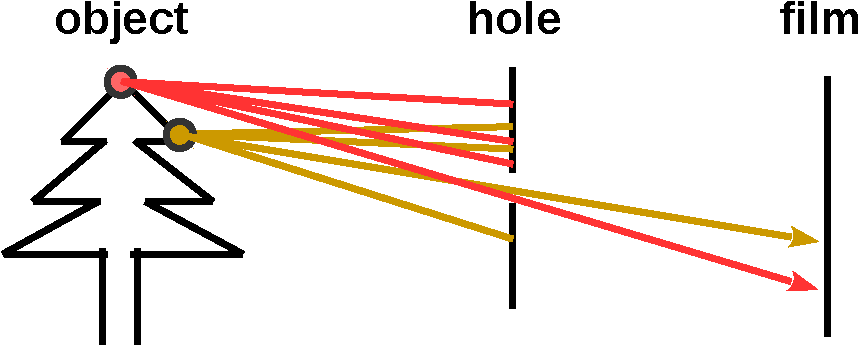
\includegraphics[width=0.9\linewidth]{./figs/hole.pdf}} \\
%	{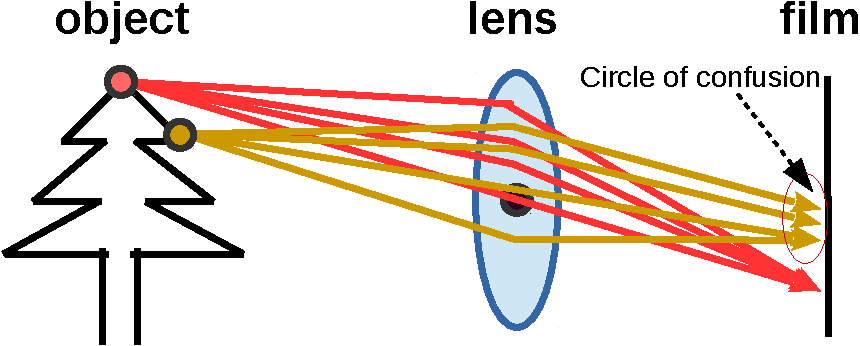
\includegraphics[width=0.9\linewidth]{./figs/lens.pdf}}
%\end{center}
%\caption{Function of the lens.}
%\end{figure}
%\end{column}
%\begin{column}{0.4\linewidth}
%\begin{itemize}
%	\item {Confusion is inevitable}
%	\item {Overall it is beter to integrate lens}
%\end{itemize}
%\end{column}
%\end{columns}
%\end{frame}
%
%\begin{frame}
% \frametitle{Basic knowledge about camera: the aperture (6)}
%\begin{figure}
%\begin{center}
%	{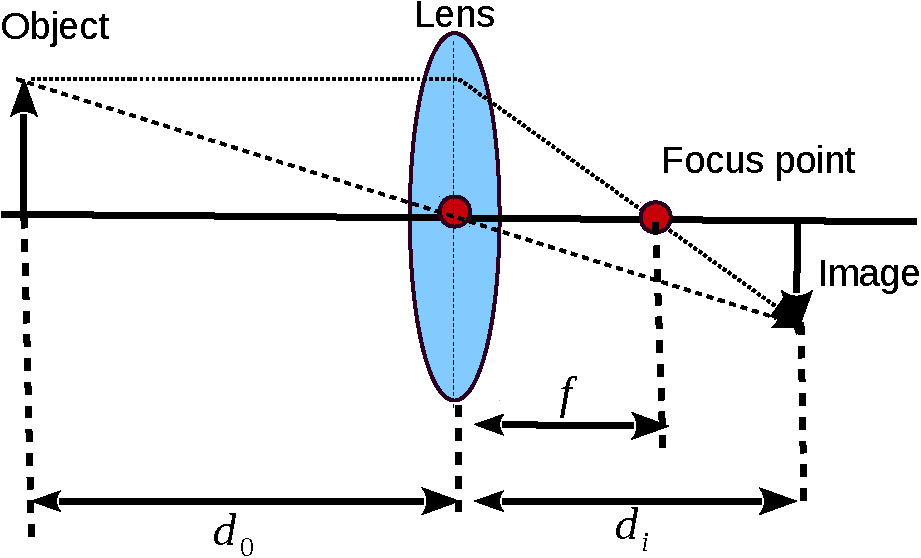
\includegraphics[width=0.6\linewidth]{./figs/lens_strct.pdf}}
%\end{center}
%\end{figure}
%\begin{itemize}
%	\item {We knew following equation in our high school}
%\end{itemize}
%\begin{equation}
%	\frac{1}{d_0}+\frac{1}{d_i}=\frac{1}{f} \nonumber
%\end{equation}
%\begin{itemize}
%	\item {When $d_0$ and $f$ are fixed, $d_i$ cannot be arbitrarily large or small}
%\end{itemize}
%\end{frame}
%
%\begin{frame}
% \frametitle{Basic knowledge about camera: the aperture (7)}
% \begin{itemize}
% 	\item {Previous equation does not hold always in practice}
% \end{itemize}
%\begin{figure}
%\begin{center}
%	\subfigure[]
%	{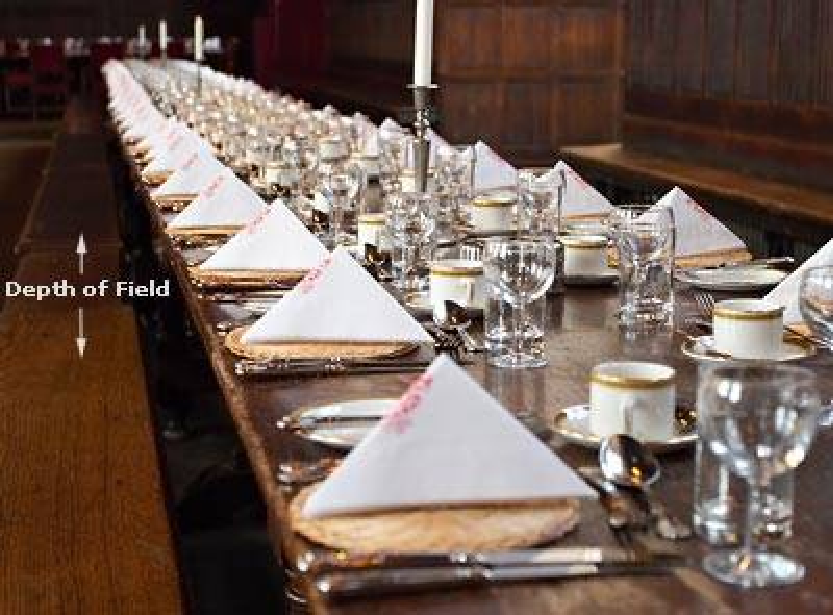
\includegraphics[width=0.48\linewidth]{./figs/depthfield1.pdf}}
%	\subfigure[]
%	{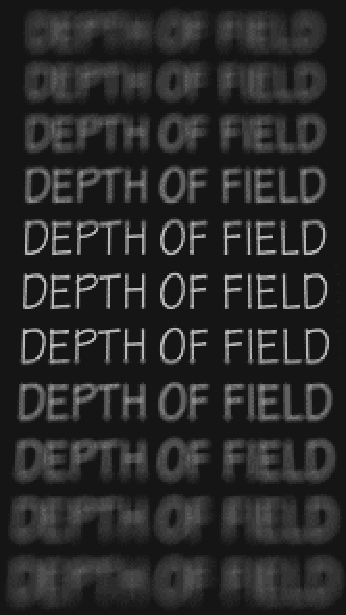
\includegraphics[width=0.20\linewidth]{./figs/depthfield2.pdf}}
%\end{center}
%\end{figure}
%\begin{itemize}
%	\item {Only certain range of ``depth of field'' is clear to us}
%\end{itemize}
%\end{frame}
%
%\begin{frame}
% \frametitle{Basic knowledge about camera: the lens (8)}
%\begin{figure}
%\begin{itemize}
%	\item {The length of focus also plays an important role}
%\end{itemize}
%\begin{center}
%	{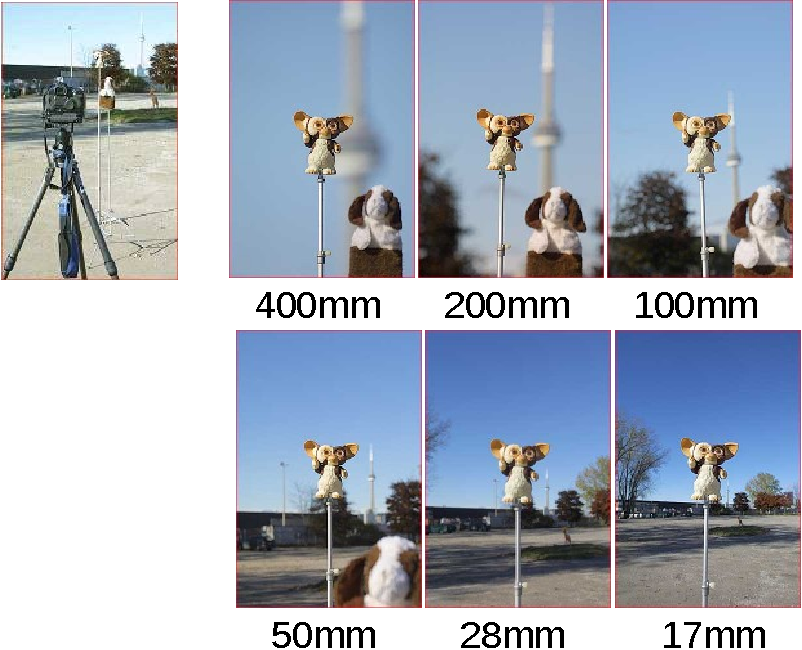
\includegraphics[width=0.5\linewidth]{./figs/longfocus.pdf}} \\
%\end{center}
%\caption{The impact of focus lens, imaging when the length of focus varies.}
%\end{figure}
%\begin{itemize}
%	\item {Large focus length compresses the depth}
%\end{itemize}
%\end{frame}

\begin{frame}
 \frametitle{Basic knowledge about camera: the aperture (1)}
\begin{figure}
\begin{center}
	{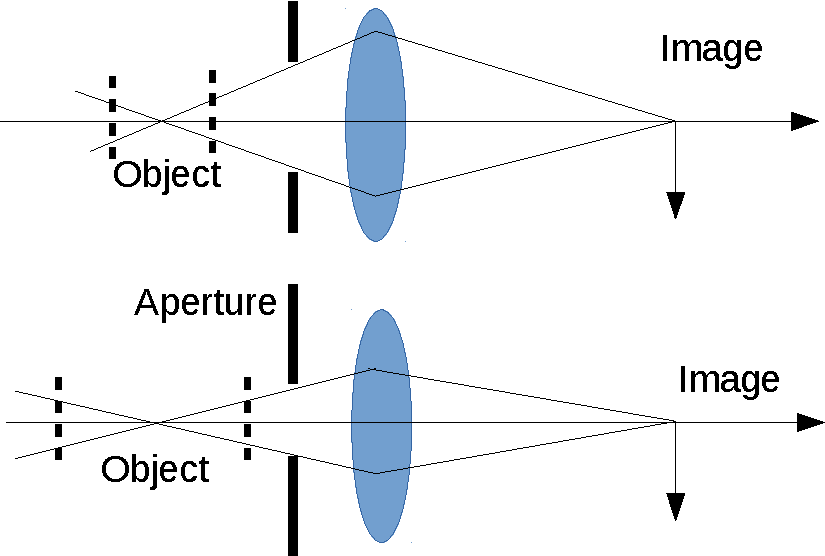
\includegraphics[width=0.55\linewidth]{./figs/apert3.pdf}}
\end{center}
\end{figure}
\begin{itemize}
	\item {Large aperture covers relatively short ``\textbf{depth of field}''}
	\item {Small aperture covers wide ``\textbf{depth of field}'' (DOF)}
	\item {However, small aperture allows less light pass-through}
	\item {It requires longer exposure time}
\end{itemize}
\end{frame}


\begin{frame}
 \frametitle{Basic knowledge about camera: the aperture (2)}
\begin{figure}
\begin{center}
	\subfigure[f=2.8, large aperture]
	{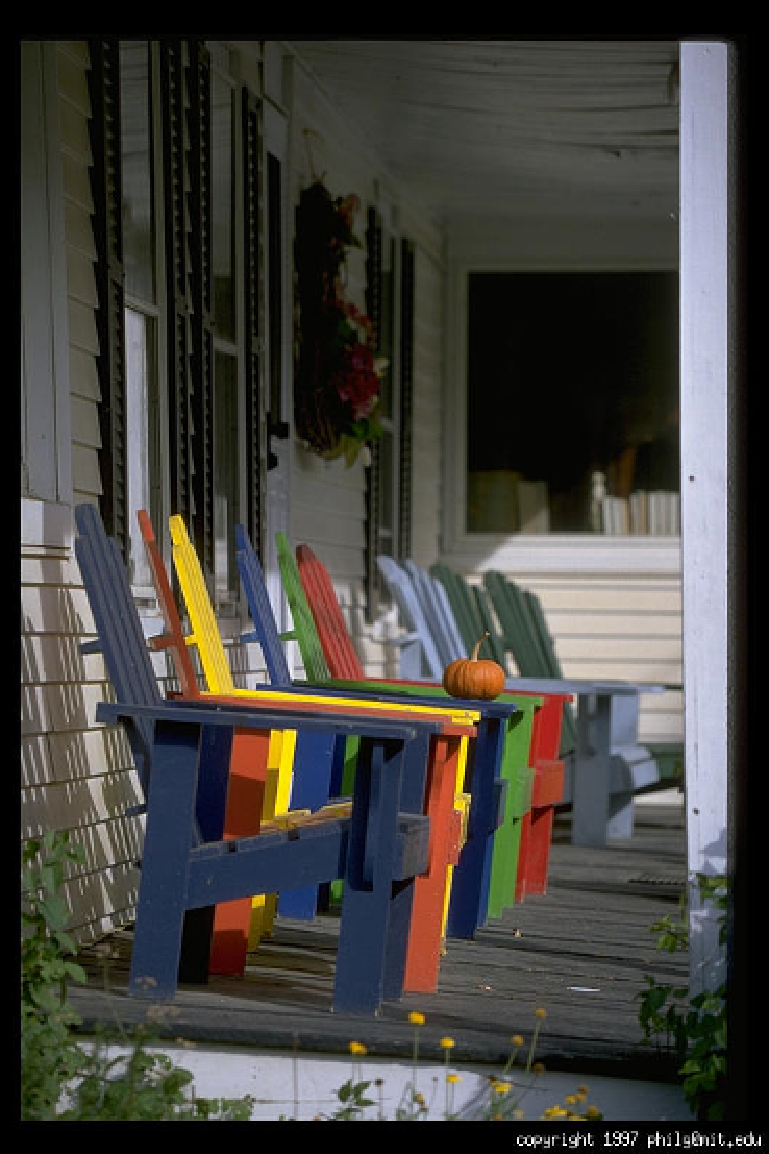
\includegraphics[width=0.30\linewidth]{./figs/apert1.pdf}}
	\hspace{0.15in}
	\subfigure[f=22, small aperture]
	{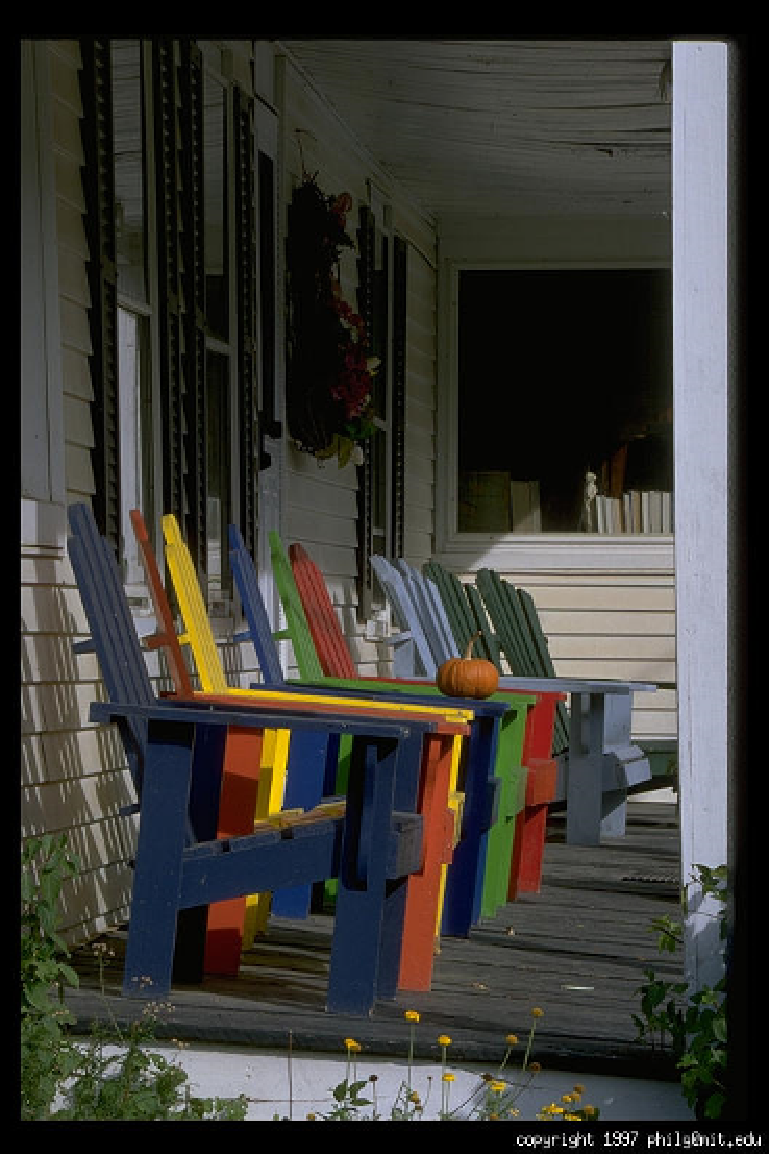
\includegraphics[width=0.30\linewidth]{./figs/apert2.pdf}}
\end{center}
\end{figure}
\begin{itemize}
	\item {Large aperture covers relatively short ``\textbf{depth of field}''}
\end{itemize}
\end{frame}
\section{Geometric Image Transformations}
\begin{frame}<beamer>
    \frametitle{Outline}
    \tableofcontents[currentsection]
\end{frame}

\begin{frame}
\frametitle {About Basic Geometric Transformations on Image}
\begin{itemize}
	\item {We already know how to process image as a multi-variable function}
	\item {We want to see how image is processed as a geometric matrix/map}
	\item {Basic linear transformations will be covered}
	\begin{itemize}
		\item {Translation}
		\item {Rotation}
		\item {Scaling}
		\item {Affine}
	\end{itemize}
\end{itemize}
\begin{figure}
	{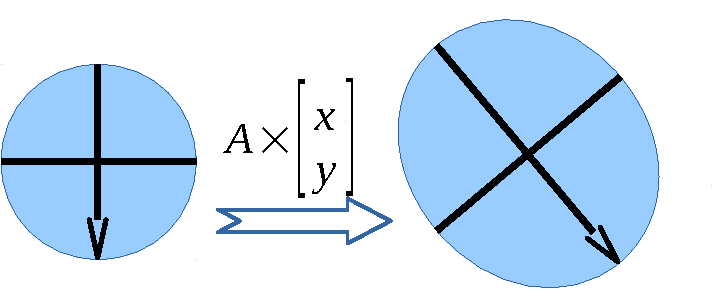
\includegraphics[width=0.5\linewidth]{./figs/imgtrans_demo.pdf}}
\end{figure}
\end{frame}

\begin{frame}
\frametitle {Image Translation}
\begin{itemize}
	\item {Move image along x, y directions or both as a whole}
\end{itemize}
\vspace{0.15in}
\begin{figure}
	{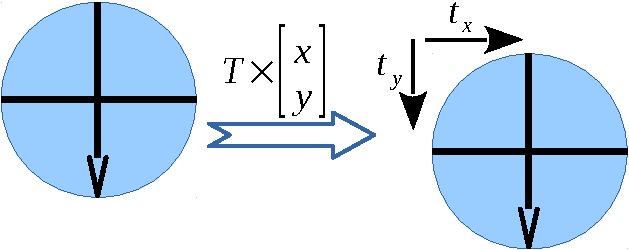
\includegraphics[width=0.6\linewidth]{./figs/imgtrans_trans.pdf}}
\end{figure}
\begin{equation}
	[x'~~y'~~1]^T= \left[ \begin{array}{ccc}
	1 & 0 & t_x \\
	0 & 1 & t_y \\
	0 & 0 & 1 
	\end{array} \right] \left[ \begin{array}{c}
	x \\
	y \\
	1
	\end{array} \right]
\end{equation}
\end{frame}

\begin{frame}
\frametitle {Image Rotation}
\begin{itemize}
	\item {Move image along x, y directions or both as a whole}
\end{itemize}
\vspace{0.1in}
\begin{figure}
	{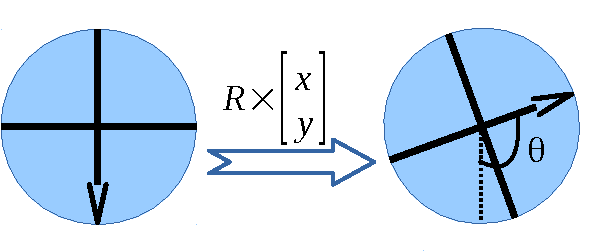
\includegraphics[width=0.6\linewidth]{./figs/imgtrans_rotate.pdf}}
\end{figure}
\begin{equation}
	[x'~~y'~~1]^T=\left[ \begin{array}{ccc}
	cos(\theta) & -sin(\theta) & 0 \\
	sin(\theta) & cos(\theta) & 0 \\
	0 & 0 & 1 
	\end{array} \right] \left[ \begin{array}{c}
	x \\
	y \\
	1
	\end{array} \right]
\end{equation}
\begin{itemize}
	\item {Notice that $R^{-1}=R^{T}$}
\end{itemize}
\end{frame}

\begin{frame}
\frametitle {Image Scaling}
\begin{itemize}
	\item {To achieve zoom-in or zoom-out effect}
\end{itemize}
\vspace{0.1in}
\begin{figure}
	{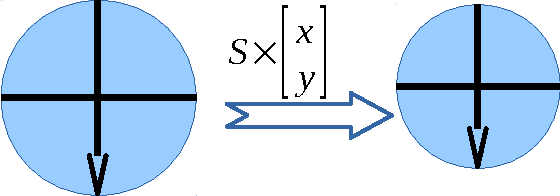
\includegraphics[width=0.6\linewidth]{./figs/imgtrans_scale.pdf}}
\end{figure}
\begin{equation}
	[x'~~y'~~1]^T= \left[ \begin{array}{ccc}
	s_x & 0 & 0 \\
	0 & s_y & 0 \\
	0 & 0 & 1 
	\end{array} \right] \left[ \begin{array}{c}
	x \\
	y \\
	1
	\end{array} \right]
\end{equation}
\begin{itemize}
	\item {Notice that the scaling factors for x and y directions, $s_x$ and $s_y$ could be different}
\end{itemize}
\end{frame}

\begin{frame}
\frametitle {Image Reflection}
\begin{itemize}
	\item {Also known as mirroring}
\end{itemize}
\vspace{0.1in}
\begin{figure}
	{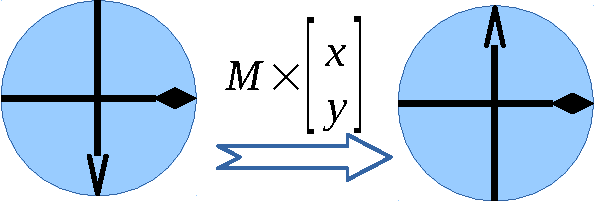
\includegraphics[width=0.55\linewidth]{./figs/imgtrans_mirr.pdf}}
	\hspace{0.15in}
	{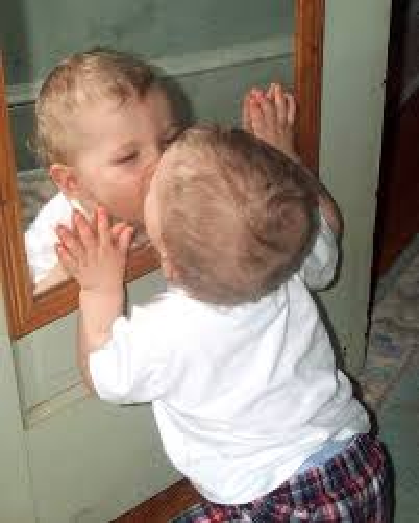
\includegraphics[width=0.15\linewidth]{./figs/mirror.pdf}}
\end{figure}
\begin{equation}
	[x'~~y'~~1]^T=\left[ \begin{array}{ccc}
	1 & 0 & 0 \\
	0 & -1 & 0 \\
	0 & 0 & 1 
	\end{array} \right] \left[ \begin{array}{c}
	x \\
	y \\
	1
	\end{array} \right]
\end{equation}
\begin{itemize}
	\item {You cannot achieve this by rotating}
	\item {If you mirror x and y both, it is then equivalent to rotating 180 degree}
\end{itemize}
\end{frame}

\begin{frame}
\frametitle {Image Affine Transformation}
\begin{itemize}
	\item {There is another one called `shear', check yourself what it is}
	\item {Basic transformations are \textbf{independent} from each other}
\end{itemize}
\vspace{0.1in}
\begin{figure}
	{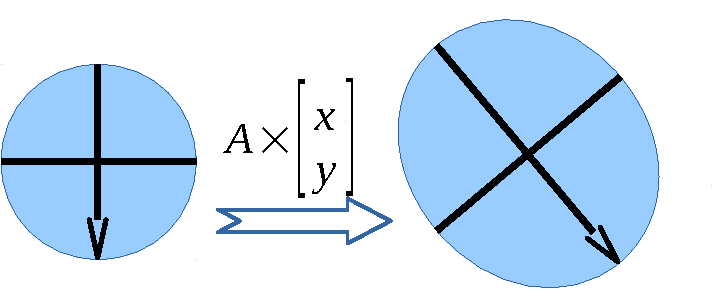
\includegraphics[width=0.6\linewidth]{./figs/imgtrans_demo.pdf}}
\end{figure}
\begin{equation}
	[x'~~y'~~1]^T= T{\cdot}S{\cdot}R{\cdot}M{\cdot}\left[ \begin{array}{c}
	x \\
	y \\
	1
	\end{array} \right]
\end{equation}
\begin{itemize}
	\item {Affine is a combination of these basic transformations}
\end{itemize}
\end{frame}

\begin{frame}
\frametitle {Geometrical Invariance (1)}
\begin{itemize}
	\item {If a vision system still recognizes what the object is after the object is geometrically transformed}
	\item {We say that this vision system is capable of geometrical invariance}
	\item {This is an IMPORTANT concept}
	\item {Our vision system is capable of geometrical invariance in various degree}
\end{itemize}

\end{frame}

\begin{frame}
\frametitle {Geometrical Invariance: rotation invariance (1)}
\begin{itemize}
	\item {How much our vision achieves rotation invariance}
\end{itemize}
\begin{figure}
	{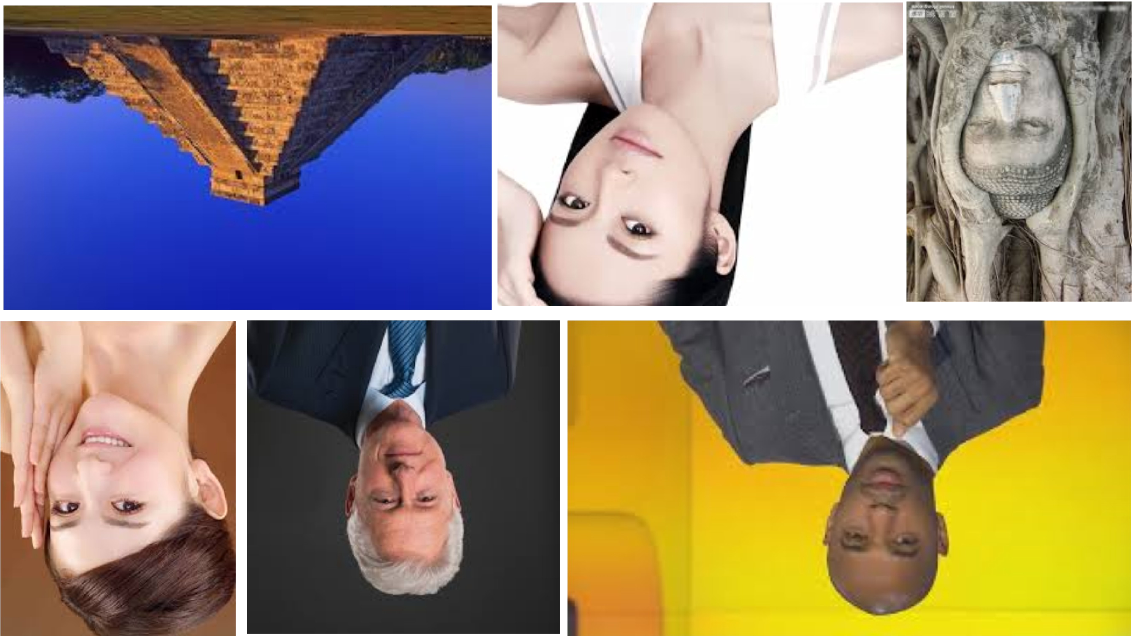
\includegraphics[width=0.75\linewidth]{./figs/invariance_rotate1.pdf}}
\end{figure}
\end{frame}

\begin{frame}
\frametitle {Geometrical Invariance: rotation invariance (2)}
\begin{itemize}
	\item {How much our vision achieves rotation invariance}
\end{itemize}
\begin{figure}
	{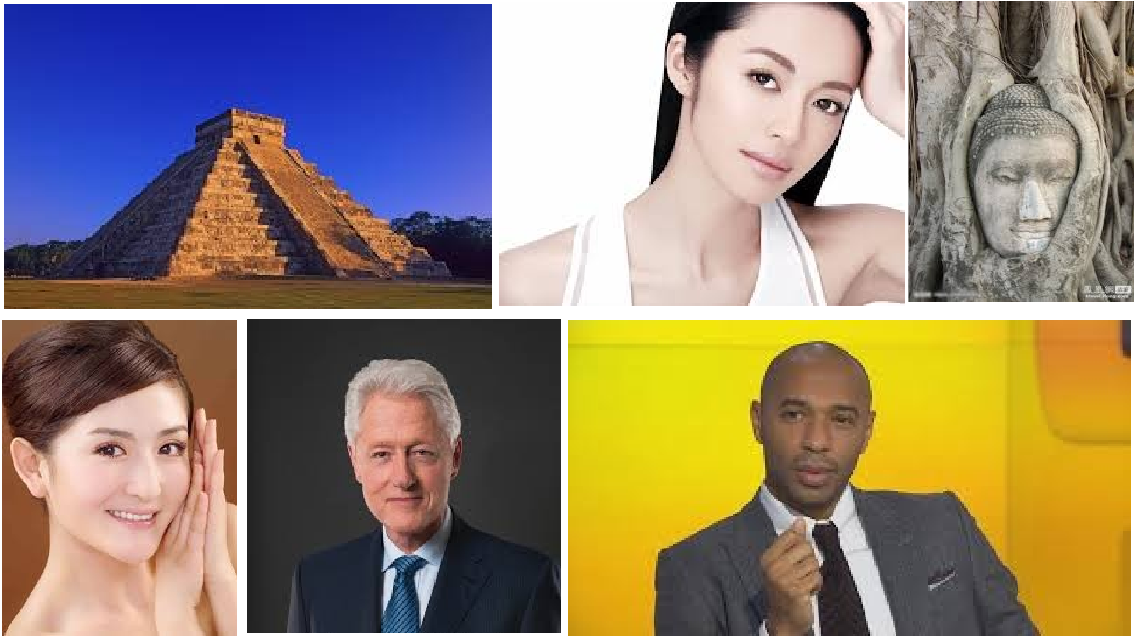
\includegraphics[width=0.75\linewidth]{./figs/invariance_rotate2.pdf}}
\end{figure}
\begin{itemize}
	\item {Verify your answer:)}
\end{itemize}
\end{frame}

\begin{frame}
\frametitle {Geometrical Invariance: scale invariance (1)}
\begin{itemize}
	\item {What you can see from the image?}
\end{itemize}
\begin{figure}
	{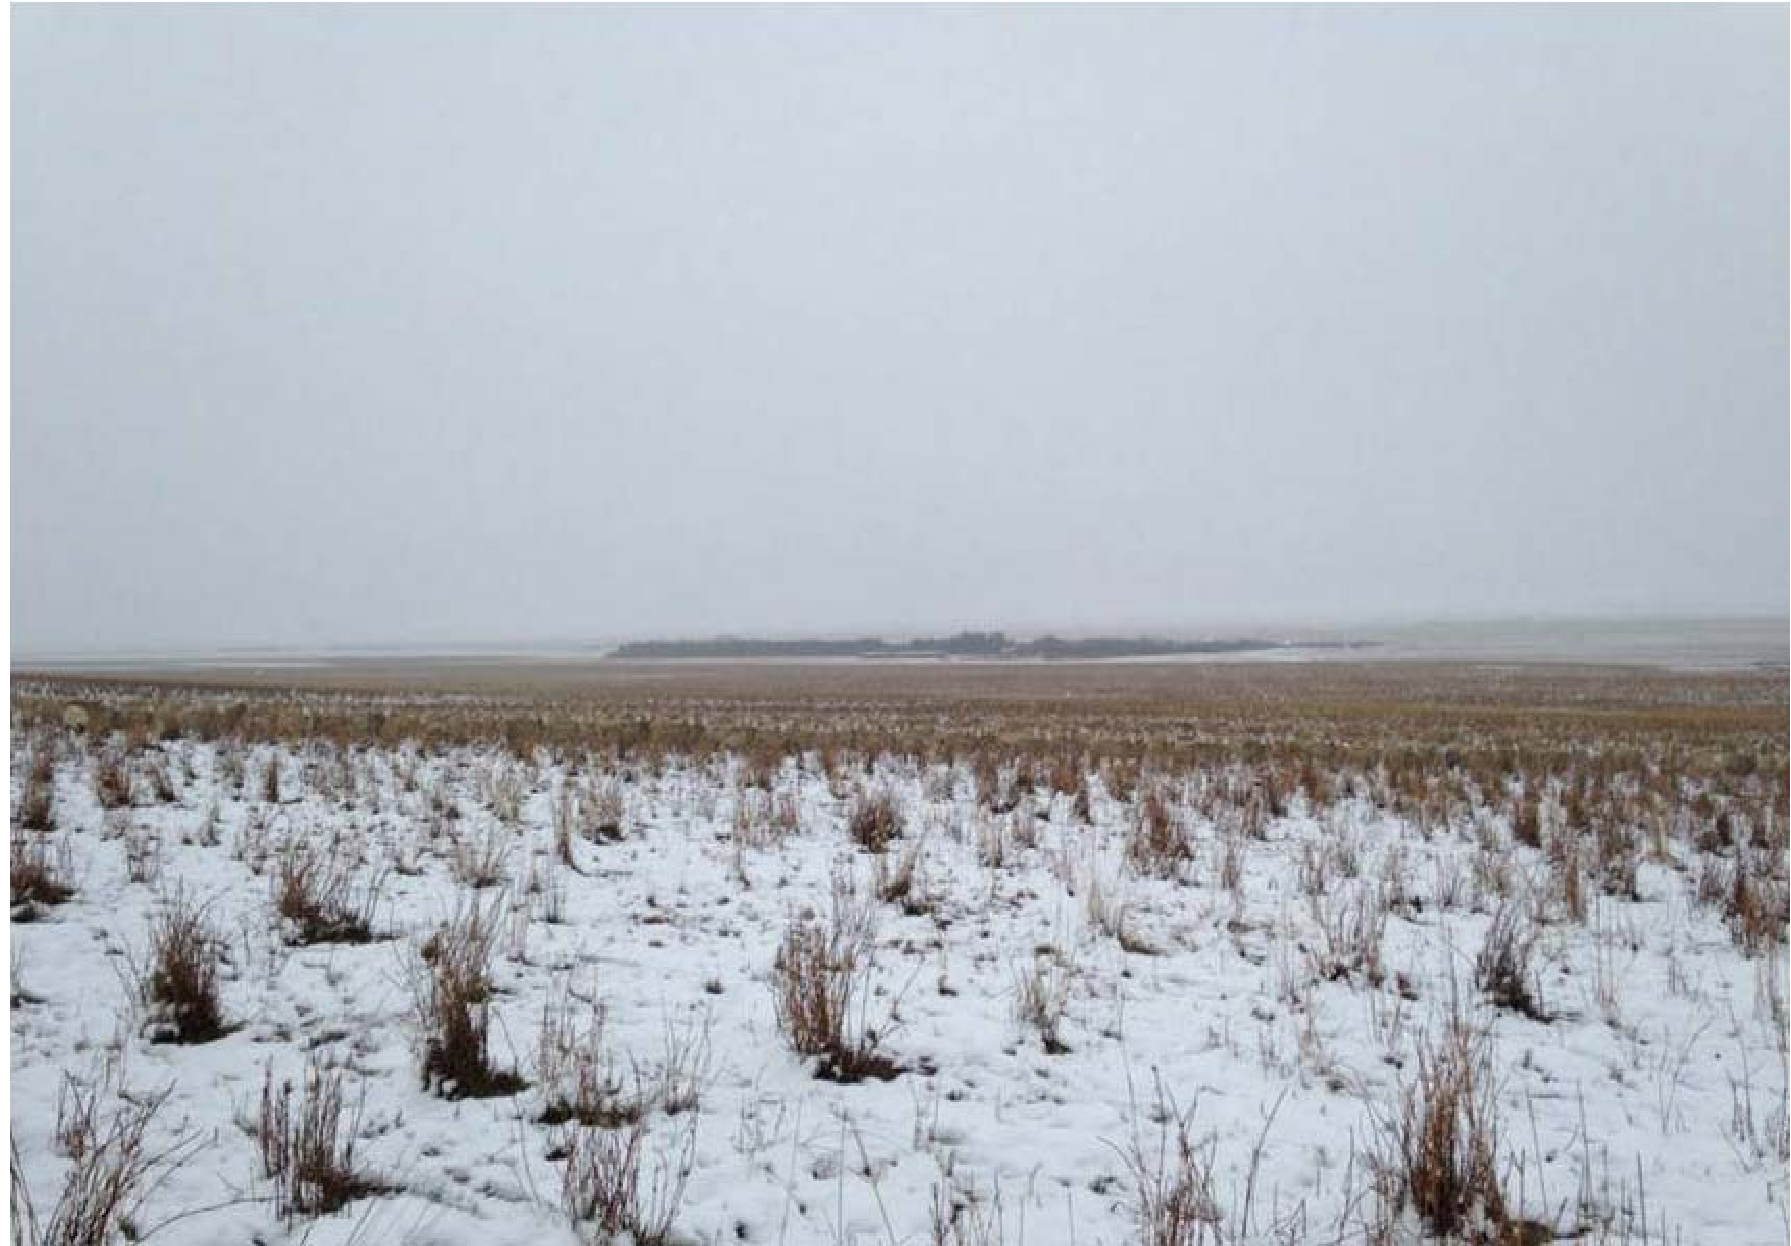
\includegraphics[width=0.7\linewidth]{./figs/scale_sheep1.pdf}}
\end{figure}
\begin{itemize}
	\item {grass, snow and ??}
\end{itemize}
\end{frame}

\begin{frame}
\frametitle {Geometrical Invariance: scale invariance (2)}
\begin{itemize}
	\item {Get closer, what you can see from the image?}
\end{itemize}
\begin{figure}
	{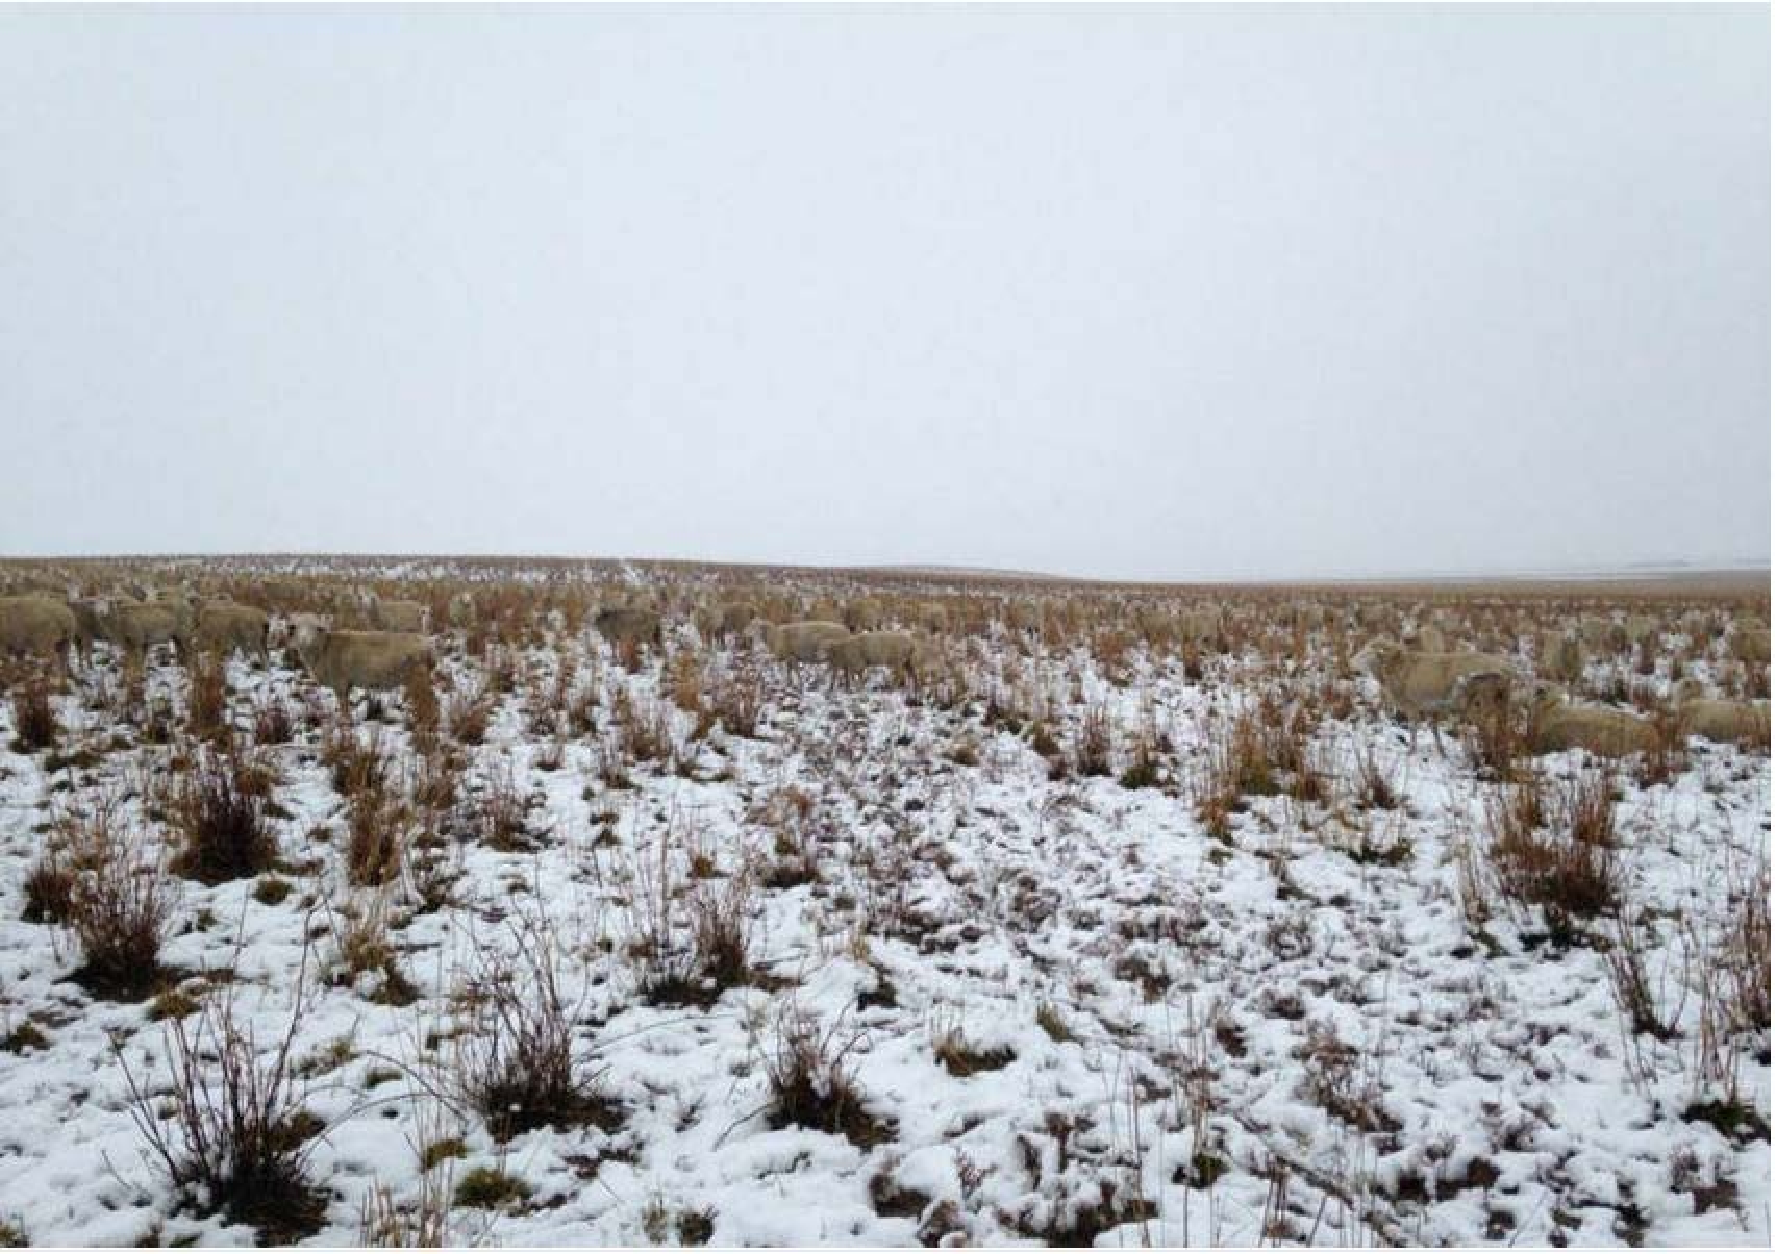
\includegraphics[width=0.65\linewidth]{./figs/scale_sheep2.pdf}}
\end{figure}
\begin{itemize}
	\item {grass, snow and ??}
\end{itemize}
\end{frame}

\begin{frame}
\frametitle {Geometrical Invariance: scale invariance (3)}
\begin{itemize}
	\item {Get closer, what you can see from the image?}
\end{itemize}
\begin{figure}
	{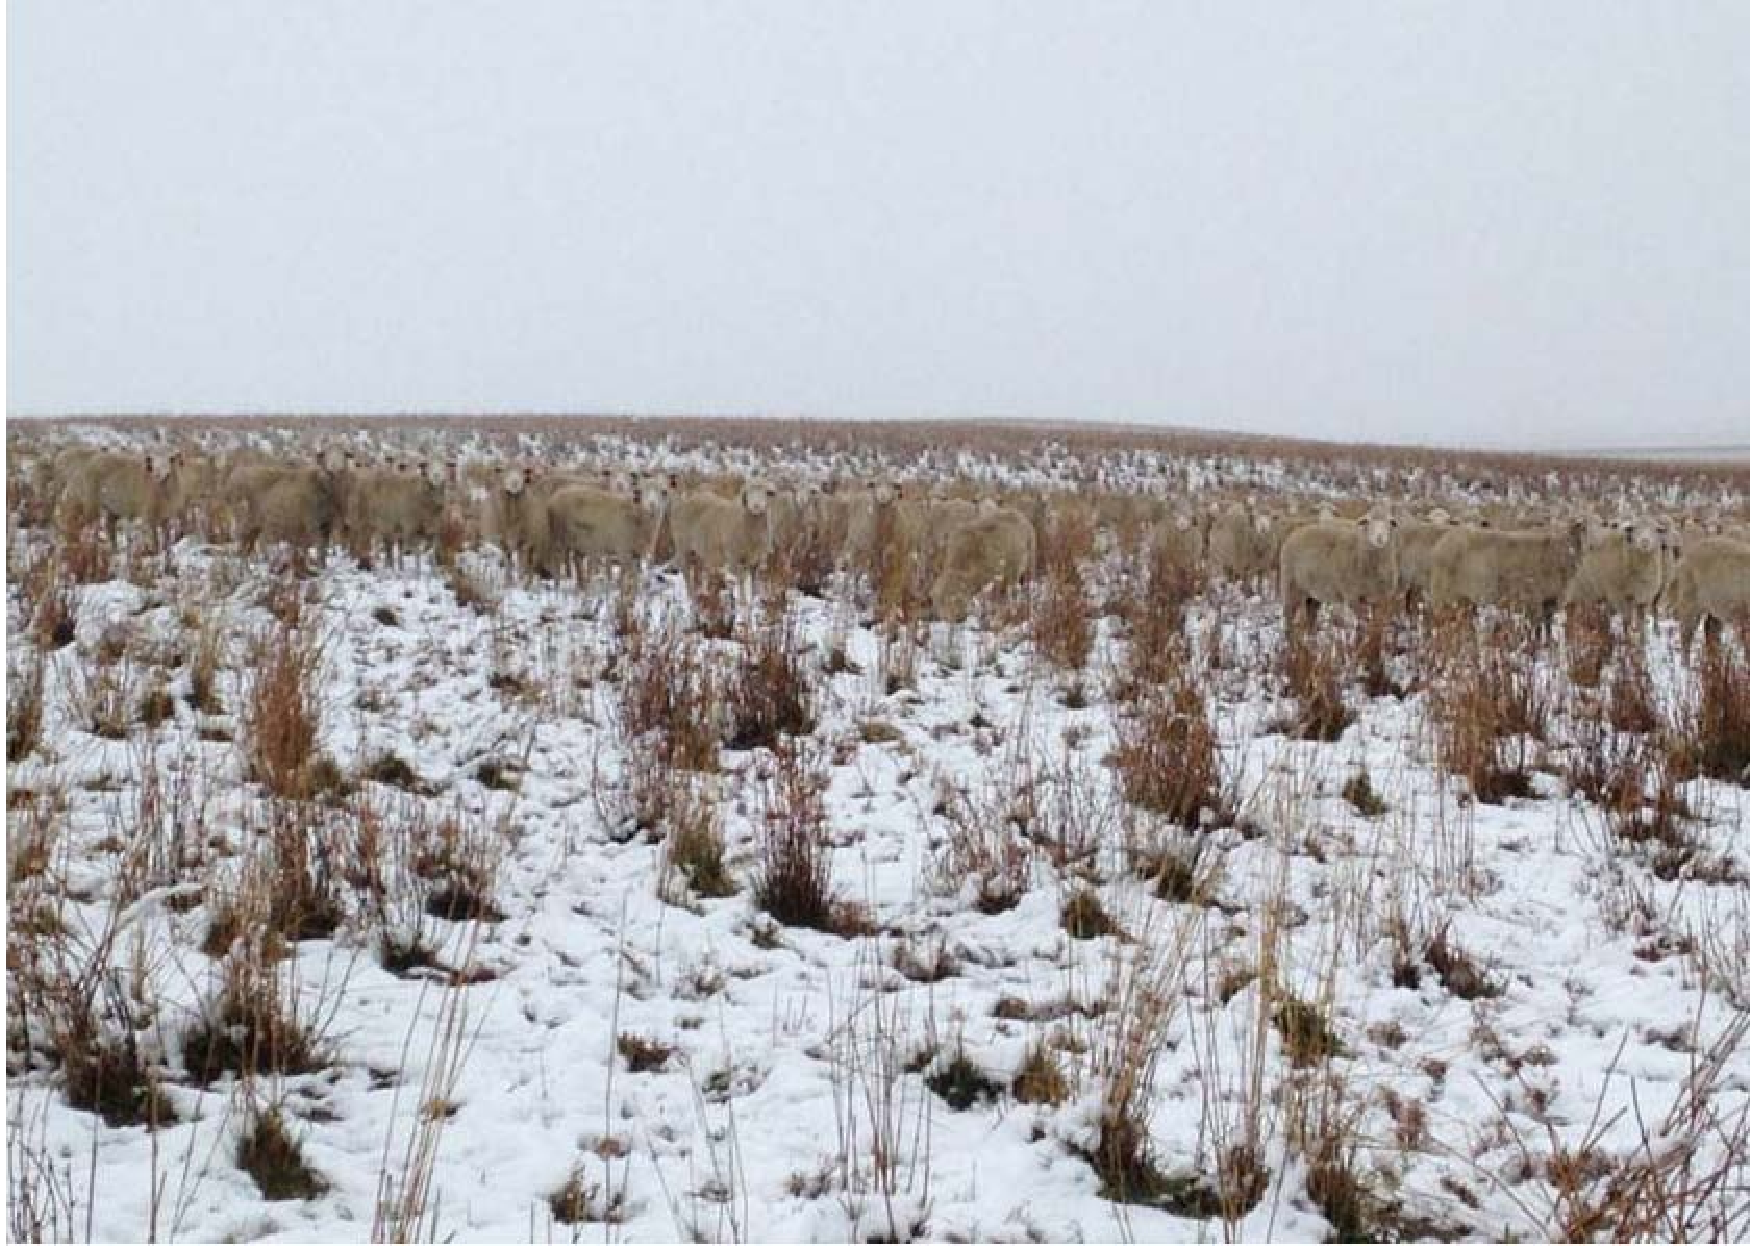
\includegraphics[width=0.65\linewidth]{./figs/scale_sheep3.pdf}}
\end{figure}
\begin{itemize}
	\item {grass, snow and sheep, clearly}
	\item {Conclusion: our vision is partially scale invariant}
\end{itemize}
\end{frame}

\begin{frame}

\frametitle {Geometrical Invariance: affine invariance (1)}
\begin{itemize}
	\item {How much our vision achieves affine invariance}
\end{itemize}
\begin{figure}
	{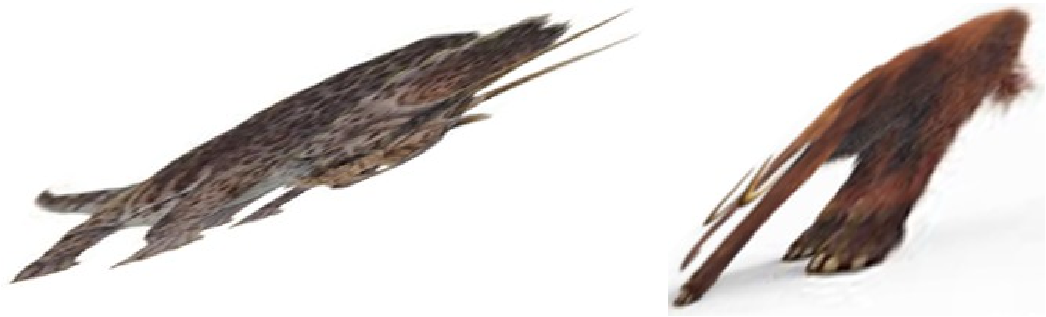
\includegraphics[width=0.75\linewidth]{./figs/invariance_affine1.pdf}}
\end{figure}
\end{frame}

\begin{frame}
\frametitle {Geometrical Invariance: affine invariance (2)}
\begin{itemize}
	\item {How much our vision achieves affine invariance}
\end{itemize}
\begin{figure}
	{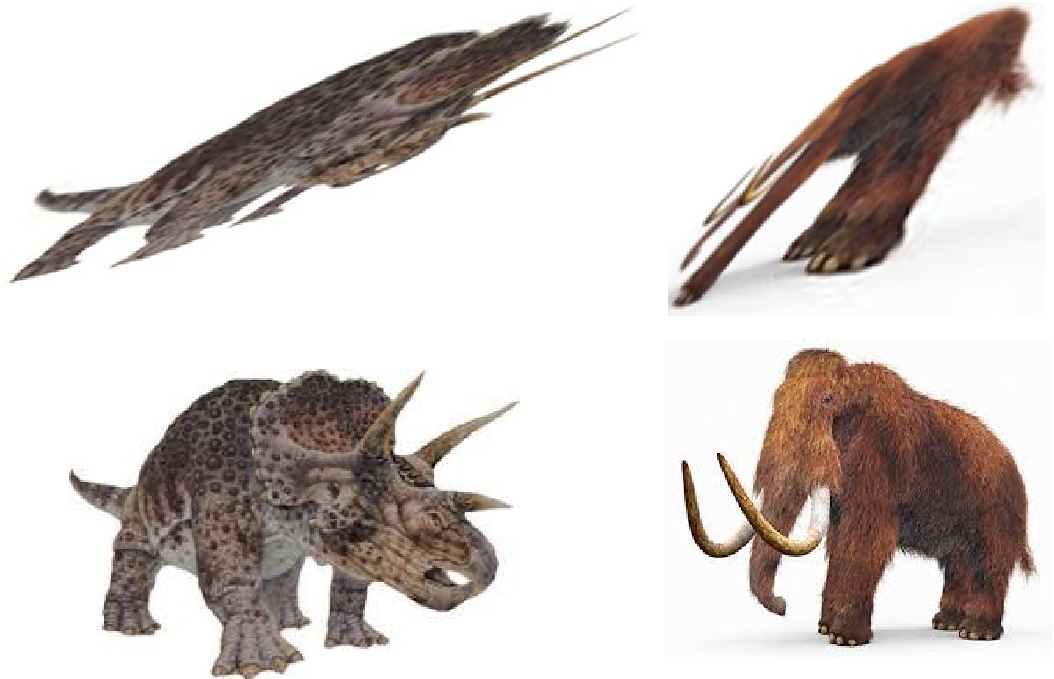
\includegraphics[width=0.75\linewidth]{./figs/invariance_affine2.pdf}}
\end{figure}
\begin{itemize}
	\item {Verify your answer:)}
\end{itemize}
\end{frame}
\input{bib.tex}
\section{}
\begin{frame}
    \begin{center}
     \vspace{1.1in}
      \Huge{Q \& A}
    \end{center}
  \end{frame}
\begin{frame}
    \begin{center}
     \vspace{1.1in}
      \Huge{Thanks for your attention!}
    \end{center}
  \end{frame}
\end{document}
